% ==============================================================================
% MAIN.TEX - Archivo Principal del Libro de Apuntes
% ==============================================================================
\documentclass[11pt, a4paper, twoside, openright]{report}

% Carga de la configuración y preámbulo estilizado
% ==============================================================================
% PREAMBLE.TEX - Configuración, Paquetes y Entornos Estilizados
% ==============================================================================

\usepackage[spanish,es-tabla]{babel}
\usepackage[utf8]{inputenc}
\usepackage[margin=2.5cm, headheight=14pt]{geometry}
\raggedbottom % Evita errores 'Underfull \vbox' equilibrando márgenes inferiores

\usepackage{amsmath, amsfonts, amssymb, amsthm, mathtools}
\usepackage{enumitem}
\usepackage{booktabs}   % Tablas de calidad editorial
\usepackage{tabularx}   % Tablas ajustables
\usepackage{microtype}  % Mejora tipográfica de justificación
\usepackage{xcolor}
\usepackage[most]{tcolorbox}
\tcbuselibrary{theorems, skins, breakable}
\usepackage{hyperref}
\usepackage{bookmark}

\usepackage{tikz}
\usetikzlibrary{babel}
\usetikzlibrary{patterns}

% Registro completo de niveles en la tabla de contenidos
\setcounter{tocdepth}{2}
\setcounter{secnumdepth}{2}

\newcounter{problemacontador}[chapter]

\newcommand{\seccionproblemas}[1][Problemas resueltos]{%
  \section{#1}%
  \setcounter{problemacontador}{0}%
}


% ------------------------------------------------------------------------------
% Paleta de Colores Académicos
% ------------------------------------------------------------------------------
\definecolor{maincolor}{RGB}{27, 54, 93}      % Azul Marino Profundo (Títulos/Encabezados)
\definecolor{accentcolor}{RGB}{0, 128, 128}    % Azul Teal / Turquesa Oscuro
\definecolor{defcolor}{RGB}{41, 128, 185}     % Azul Definición
\definecolor{conceptcolor}{RGB}{31, 78, 121}   % Azul Concepto Clave
\definecolor{excolor}{RGB}{39, 174, 96}       % Verde Ejemplo Resuelto
\definecolor{notecolor}{RGB}{142, 68, 173}    % Morado Nota / Observación
\definecolor{bglight}{RGB}{248, 249, 250}     % Fondo neutro claro
\definecolor{boxbg}{RGB}{245, 247, 250}       % Fondo claro para cajas

% ------------------------------------------------------------------------------
% Configuración de Hyperref
% ------------------------------------------------------------------------------
\hypersetup{
    colorlinks=true,
    linkcolor=maincolor,
    citecolor=accentcolor,
    urlcolor=accentcolor,
    pdfstartview=FitH
}

% ------------------------------------------------------------------------------
% Configuración de Encabezados y Pies a Doble Cara (fancyhdr)
% ------------------------------------------------------------------------------
\usepackage{fancyhdr}
\pagestyle{fancy}
\fancyhf{} 

% Páginas Pares (Izquierda / Left): Capítulo a la izq, Número de página a la der.
\fancyhead[LE]{\small\bfseries\color{maincolor}\leftmark}
\fancyhead[RE]{\small\bfseries\color{maincolor}\thepage}

% Páginas Impares (Derecha / Right): Número de página a la izq, Sección a la der.
\fancyhead[LO]{\small\bfseries\color{maincolor}\thepage}
\fancyhead[RO]{\small\bfseries\color{maincolor}\rightmark}

\renewcommand{\chaptermark}[1]{\markboth{\thechapter.\ #1}{}}
\renewcommand{\sectionmark}[1]{\markright{\thesection.\ #1}}
\renewcommand{\headrulewidth}{0.4pt}

% Estilo plano para portadas e inicios de capítulo
\fancypagestyle{plain}{
  \fancyhf{}
  \fancyfoot[C]{\thepage}
  \renewcommand{\headrulewidth}{0pt}
}

% ------------------------------------------------------------------------------
% Entornos Estilizados (tcolorbox)
% ------------------------------------------------------------------------------

% 1. Entorno Definición
\newtcolorbox[auto counter, number within=chapter]{definicion}[1][]{%
  enhanced,
  breakable,
  colback=bglight,
  colframe=defcolor,
  fonttitle=\bfseries\color{white},
  title={Definición \thetcbcounter\if\relax\detokenize{#1}\relax\else\ (#1)\fi},
  attach boxed title to top left,
  boxed title style={colback=defcolor, sharp corners},
  arc=2pt,
  boxrule=0.8pt,
  top=8pt, bottom=8pt, left=10pt, right=10pt
}

% 2. Entorno Concepto / Principio Clave
\newtcolorbox[auto counter, number within=chapter]{concepto}[1][]{%
  enhanced,
  breakable,
  colback=maincolor!4!white,
  colframe=conceptcolor,
  fonttitle=\bfseries\color{white},
  title={Principio Fundamental \thetcbcounter\if\relax\detokenize{#1}\relax\else\ (#1)\fi},
  attach boxed title to top left,
  boxed title style={colback=conceptcolor, sharp corners},
  arc=2pt,
  boxrule=0.8pt,
  top=8pt, bottom=8pt, left=10pt, right=10pt
}

% 3. Entorno Ejemplo Resuelto
\newtcolorbox[auto counter, number within=chapter]{ejemplo}[1][]{%
  enhanced,
  breakable,
  colback=excolor!4!white,
  colframe=excolor,
  fonttitle=\bfseries\color{white},
  title={Ejemplo Resuelto \thetcbcounter\if\relax\detokenize{#1}\relax\else\ (#1)\fi},
  attach boxed title to top left,
  boxed title style={colback=excolor, sharp corners},
  arc=2pt,
  boxrule=0.8pt,
  top=8pt, bottom=8pt, left=10pt, right=10pt
}

% 4. Entorno Observación / Nota Técnica
\newtcolorbox{observacion}[1][Observación]{%
  enhanced,
  breakable,
  colback=notecolor!4!white,
  colframe=notecolor,
  fonttitle=\bfseries\color{white},
  title={#1},
  attach boxed title to top left,
  boxed title style={colback=notecolor, sharp corners},
  arc=2pt,
  boxrule=0.8pt,
  top=8pt, bottom=8pt, left=10pt, right=10pt
}

% ------------------------------------------------------------------------------
% Entorno para Problemas de la Lista del Profesor
% ------------------------------------------------------------------------------
% 8. PROBLEMA RESUELTO (Púrpura)
\newtcolorbox{problema}[1][]{
  enhanced,
  breakable,
  colback=boxbg,
  colframe=maincolor,
  fonttitle=\bfseries,
  coltitle=white,
  arc=2mm,
  boxrule=1pt,
  code={\refstepcounter{problemacontador}},
  title={Problema~\theproblemacontador\ifstrempty{#1}{}{: #1}},
  lower separated=true
}

% ------------------------------------------------------------------------------
% Macros y Comandos de Física de Partículas
% ------------------------------------------------------------------------------
\newcommand{\eV}{\text{ eV}}
\newcommand{\keV}{\text{ keV}}
\newcommand{\MeV}{\text{ MeV}}
\newcommand{\GeV}{\text{ GeV}}
\newcommand{\TeV}{\text{ TeV}}
\newcommand{\fm}{\text{ fm}}
\newcommand{\SU}[1]{\text{SU}(#1)}
\newcommand{\U}[1]{\text{U}(#1)}
\newcommand{\SO}[1]{\text{SO}(#1)}
\newcommand{\bra}[1]{\langle #1 |}
\newcommand{\ket}[1]{| #1 \rangle}
\newcommand{\bracket}[2]{\langle #1 | #2 \rangle}

\begin{document}

% ------------------------------------------------------------------------------
% Portada Académica
% ------------------------------------------------------------------------------
\begin{titlepage}
    \centering
    \vspace*{2cm}
    
    {\Huge \bfseries \color{maincolor} FÍSICA NUCLEAR Y DE PARTÍCULAS \par}
    \vspace{0.6cm}
    {\Large \scshape Prometeo 137 \par}
    
    \vspace{1.5cm}
    \color{maincolor}\rule{\linewidth}{0.8mm}
    \vfill
    
    \begin{minipage}{0.45\textwidth}
        \begin{flushleft} \large
            \emph{Asignatura:}\\
            Física Nuclear y de Partículas
        \end{flushleft}
    \end{minipage}
    ~
    \begin{minipage}{0.45\textwidth}
        \begin{flushright} \large
            \emph{Nivel:}\\
            Cuarto Curso
        \end{flushright}
    \end{minipage}
    
    \vspace{2cm}
    {\small \today \par}
\end{titlepage}

% ------------------------------------------------------------------------------
% Índices del Libro
% ------------------------------------------------------------------------------
\pagenumbering{roman}
\tableofcontents
\cleardoublepage

\pagenumbering{arabic}

% ------------------------------------------------------------------------------
% Bloque de Capítulos
% ------------------------------------------------------------------------------

% !TEX root = ../main.tex
% ==============================================================================
% TEMA 1: CONCEPTO DE PARTÍCULA FUNDAMENTAL: CLASIFICACIÓN
% ==============================================================================

\chapter{Concepto de Partícula Fundamental: Clasificación}
\label{chap:tema1}

% ==============================================================================
% SECCIÓN 1: CLASIFICACIÓN DE PARTÍCULAS FUNDAMENTALES
% ==============================================================================

\section{Clasificación de Partículas Fundamentales}

El estudio de la física subatómica requiere un esquema de clasificación sistemático para las partículas conocidas. Esta división se realiza fundamentalmente bajo dos criterios independientes: el comportamiento cuántico y estadístico (determinado por el espín) y el tipo de interacciones en las que participan.

\subsection{Criterios de Clasificación General}

\begin{concepto}[Clasificación por Espín: Fermiones vs. Bosones]
De acuerdo con el \textbf{Teorema Espín-Estadística}, toda partícula subatómica pertenece a una de las siguientes dos categorías:
\begin{itemize}
    \item \textbf{Fermiones} (espín semientero: $s = 1/2, 3/2, \dots$): Constituyen la materia. Obedecen la estadística de Fermi-Dirac y el principio de exclusión de Pauli. Sus campos anticonmutan.
    \item \textbf{Bosones} (espín entero: $s = 0, 1, 2, \dots$): Mediadores de interacciones (o escalares como el Higgs). Obedecen la estadística de Bose-Einstein y no están sujetos al principio de exclusión. Sus campos conmutan.
\end{itemize}
\end{concepto}

Por otro lado, según la respuesta ante las fuerzas fundamentales, las partículas que forman la materia se dividen en:
\begin{enumerate}[label=\alph*)]
    \item \textbf{Leptones:} Fermiones elementales (sin estructura interna apreciable) que no experimentan la interacción fuerte.
    \item \textbf{Hadrones:} Partículas compuestas por constituyentes con carga de color (quarks y antiquarks). Su característica definitoria es que experimentan la interacción fuerte, además de la electromagnética y la débil si sus componentes o la partícula global poseen las cargas correspondientes.
\end{enumerate}

---

\subsection{Estructura Hadrónica: Hadrones Convencionales y Exóticos}

Dado que la interacción fuerte se describe mediante la Cromodinámica Cuántica (QCD) bajo el grupo de simetría gauge $\SU{3}_C$, los estados ligados de quarks que observamos en la naturaleza deben ser invariantes de color (singletes de color o ``materia blanca''). 

La condición de invarianza gauge de color establece que la composición de cualquier hadrón en términos de contenido de quarks ($q$) y antiquarks ($\bar{q}$) responde a la fórmula general:

\begin{equation}
\label{eq:hadron_formula}
(q q q)^m \, (q \bar{q})^n \quad \text{con } m, n \in \mathbb{N}_0 = \{0, 1, 2, 3, \dots\}
\end{equation}

Donde el término $(qqq)$ representa un trío con combinación totalmente antisimétrica de color ($\epsilon_{ijk} q_i q_j q_k$), y $(q\bar{q})$ representa un par quark-antiquark neutro de color ($\delta_{ij} q_i \bar{q}_j$).

\begin{table}[h!]
\centering
\caption{Clasificación del espectro hadrónico según su contenido de quarks.}
\label{tab:hadron_classification}
\vspace{0.3cm}
\small
\begin{tabularx}{\linewidth}{c c X l c c}
\toprule
\textbf{$m$} & \textbf{$n$} & \textbf{Configuración} & \textbf{Denominación} & \textbf{Espín ($s$)} & \textbf{Ejemplos Destacados} \\
\midrule
1 & 0 & $q q q$ & \textbf{Barión} (Convencional) & Semientero & Protón ($uud$), Neutrón ($udd$), $\Lambda^0$ ($uds$) \\
0 & 1 & $q \bar{q}$ & \textbf{Mesón} (Convencional) & Entero & Pión ($\pi^+ = u\bar{d}$), Kaón ($K^0 = d\bar{s}$) \\
\midrule
0 & 2 & $q \bar{q} q \bar{q}$ & \textbf{Tetraquark} (Exótico) & Entero & $X(3872)$, $Z_c(3900)$ \\
1 & 1 & $q q q q \bar{q}$ & \textbf{Pentaquark} (Exótico) & Semientero & $P_c^+(4380)$, $P_c^+(4450)$ \\
2 & 0 & $q q q q q q$ & \textbf{Hexaquark / Dibarión} & Entero & Deuterón ($pn$), Resonancia $d^*(2380)$ \\
\bottomrule
\end{tabularx}
\end{table}

\begin{observacion}[Hadrones Exóticos]
Los estados con $m+n > 1$ se denominan \textbf{hadrones exóticos}. Aunque la teoría de QCD predijo su existencia teórica desde el modelo de Gell-Mann (1964), su confirmación experimental definitiva ha tenido lugar en las últimas dos décadas en experimentos de altas energías como LHCb, Belle y BESIII.
\end{observacion}

---

\subsection{Interacciones en Hadrones y Criterios de Selección}

Dado que los quarks que constituyen a los hadrones poseen:
\begin{enumerate}[label=\roman*)]
    \item \textbf{Carga de Color:} Interactúan mediante la interacción fuerte.
    \item \textbf{Carga Eléctrica ($Q \ne 0$):} Interactúan mediante la interacción electromagnética.
    \item \textbf{Isospín Débil ($T_3$):} Interactúan mediante la interacción débil.
\end{enumerate}

En principio, las tres interacciones pueden intervenir en las reacciones o desintegraciones entre hadrones. Sin embargo, el mecanismo dominante queda determinado por las leyes de conservación de números cuánticos y las escalas características de tiempo de cada interacción.

\begin{table}[h!]
\centering
\caption{Escalas de tiempo y conservación de sabor en interacciones hadrónicas.}
\label{tab:interacciones_tiempos}
\vspace{0.2cm}
\small
\begin{tabularx}{\linewidth}{l c X}
\toprule
\textbf{Interacción} & \textbf{Tiempo Característico ($\tau$)} & \textbf{Conservación de Sabor ($S, C, B, T$)} \\
\midrule
\textbf{Fuerte} & $10^{-24} - 10^{-23} \text{ s}$ & Estrictamente conservado ($\Delta S = 0$). \\
\textbf{Electromagnética} & $10^{-21} - 10^{-16} \text{ s}$ & Estrictamente conservado ($\Delta S = 0$). \\
\textbf{Débil} & $10^{-13} - 10^{-8} \text{ s}$ & Puede violar el sabor ($\Delta S = \pm 1$). \\
\bottomrule
\end{tabularx}
\end{table}

\newpage
\subsection{Análisis Detallado de un Proceso: La Desintegración $\Lambda^0 \to p + \pi^-$}

Consideremos el proceso de desintegración del hiperón neutral $\Lambda^0$:
\begin{equation}
\label{eq:lambda_decay}
\Lambda^0 \longrightarrow p + \pi^-
\end{equation}

\subsubsection*{1. Identificación del contenido de quarks y cargas}
\begin{itemize}
    \item \textbf{Estado Inicial:} $\Lambda^0 = (u\,d\,s)$ --- Barión neutro con extrañeza $S = -1$.
    \item \textbf{Estado Final:} 
    \begin{itemize}
        \item Protón $p = (u\,u\,d)$ --- Barión cargado ($Q = +1$) con extrañeza $S = 0$.
        \item Pión $\pi^- = (d\,\bar{u})$ --- Mesón cargado ($Q = -1$) con extrañeza $S = 0$.
    \end{itemize}
\end{itemize}

\subsubsection*{2. Análisis de las interacciones posibles}
Aunque todas las partículas involucradas ($\Lambda^0, p, \pi^-$) son hadrones que cargan interacción fuerte, electromagnética y débil:
\begin{itemize}
    \item \textbf{¿Puede ser Interacción Fuerte?} \\
    La extrañeza inicial es $S_{\text{inicial}} = -1$, mientras que la final es $S_{\text{final}} = 0 + 0 = 0$. Hubo un cambio de extrañeza de $\Delta S = +1$. La interacción fuerte conserva estrictamente el sabor, por lo que no puede mediar este proceso.
    
    \item \textbf{¿Puede ser Interacción Electromagnética?} \\
    La interacción electromagnética también conserva el sabor ($\Delta S = 0$). Por lo tanto, queda descartada.
    
    \item \textbf{¿Por qué es una Interacción Débil?} \\
    La interacción débil es la única fuerza del Modelo Estándar que permite transiciones entre familias de quarks (violación del sabor con $\Delta S = \pm 1$) mediante el intercambio de bosones cargados $W^\pm$. En este proceso, el quark $s$ ($Q=-1/3$) se transforma en un quark $u$ ($Q=+2/3$) emitiendo un bosón $W^-$, el cual se desintegra posteriormente en un par $d\,\bar{u}$ ($\pi^-$):
    $$s \longrightarrow u + W^- \longrightarrow u + (d\,\bar{u})$$
\end{itemize}

\begin{ejemplo}[Conclusión sobre la Vida Media del $\Lambda^0$]
Debido a que el proceso $\Lambda^0 \to p + \pi^-$ transcurre obligatoriamente a través de la \textbf{interacción débil}, su vida media medida experimentalmente es de:
$$\tau_{\Lambda^0} \approx 2.63 \times 10^{-10} \text{ s}$$
Este tiempo es enormemente mayor que el tiempo característico de una desintegración fuerte ($\sim 10^{-23} \text{ s}$), lo cual constituye la evidencia experimental directa de que el proceso es guiado por la fuerza débil.
\end{ejemplo}

\newpage
% ==============================================================================
% SUBSECCIÓN: EL DESCUBRIMIENTO DEL MUÓN Y LA FÍSICA DE RAYOS CÓSMICOS
% ==============================================================================

\subsection{El Descubrimiento del Muón y la Física de Rayos Cósmicos}

A principios de la década de 1930, el esquema de partículas elementales parecía completo con el electrón ($e^-$), el protón ($p$), el neutrón ($n$), el fotón ($\gamma$) y la hipótesis del neutrino ($\nu$). Sin embargo, el estudio de la radiación cósmica mediante cámaras de niebla puestas en campos magnéticos reveló la existencia de nuevas entidades subatómicas.

En 1937, Seth H. Neddermeyer y Carl D. Anderson descubrieron en los rayos cósmicos una partícula cargada cuya masa se situaba en un rango intermedio entre la del electrón y la del protón.

\subsubsection{Mecanismos de Pérdida de Energía de Partículas Cargadas en la Materia}

Para entender el experimento fundamental de Neddermeyer y Anderson, es necesario analizar cómo interaccionan las partículas cargadas al atravesar un medio absorbente:

\begin{enumerate}[label=\arabic*)]
    \item \textbf{Pérdida por Ionización y Excitación (Fórmula de Bethe-Bloch):} \\
    Las partículas cargadas transfieren energía a los electrones atómicos del medio mediante colisiones inelásticas. La pérdida específica de energía por unidad de longitud viene dada por:
    \begin{equation}
    -\left(\frac{dE}{dx}\right)_{\text{ion}} \propto \frac{z^2}{\beta^2} \ln \left( \frac{2 m_e c^2 \beta^2 \gamma^2 T_{\text{máx}}}{I^2} \right)
    \end{equation}
    donde $z e$ es la carga de la partícula incidente, $\beta = v/c$ su velocidad y $I$ el potencial medio de ionización del medio. Para partículas ultra-relativistas ($\beta \approx 1$), la ionización alcanza un mínimo de pérdida (\emph{partículas de ionización mínima} o MIPs).
    
    \item \textbf{Pérdida por Radiación de Frenado (\emph{Bremsstrahlung}):} \\
    Cuando una partícula cargada se desacelera en el campo eléctrico de los núcleos del absorbente, emite fotones. La pérdida de energía por radiación es inversamente proporcional al cuadrado de la masa de la partícula:
    \begin{equation}
    -\left(\frac{dE}{dx}\right)_{\text{rad}} \propto \frac{Z^2 e^6}{m^2 c^4} E
    \end{equation}
    Para el electrón ($m = m_e$), la emisión de \emph{Bremsstrahlung} es el mecanismo dominante a altas energías ($E > 10 \text{ MeV}$ en plomo), produciendo cascadas o lluvias electromagnéticas ($\text{showers}$). En cambio, para una partícula de mayor masa, este efecto queda severamente suprimido por un factor $(m_e/m)^2$.
\end{enumerate}

\newpage
%-------------------------------------
\subsubsection{El Experimento de Neddermeyer y Anderson (1937)}

Neddermeyer y Anderson operaron una cámara de niebla sumergida en un campo magnético de intensidad conocida e introdujeron en su centro una placa pesada de platino de $1\text{ cm}$ de espesor (equivalente en densidad electrónica a $1.96\text{ cm}$ de plomo).

Al medir la rigidez magnética ($B\rho$) antes y después de atravesar la placa, calcularon la pérdida fraccionaria de energía $\Delta E / E_i$ para más de 6000 trazas de rayos cósmicos con energías por debajo de $500\text{ MeV}$.

\begin{center}
\begin{tikzpicture}[scale=0.95]
  % Ejes
  \draw[->, thick] (0,0) -- (6.5,0) node[right] {$E_i \text{ (MeV)}$};
  \draw[->, thick] (0,0) -- (0,4.5) node[above] {$-\Delta E / d \text{ (MeV/cm)}$};
  
  % Línea del límite teórica Bethe-Heitler (\Delta E / E = 1)
  \draw[thick, gray, dashed] (0,0) -- (5.5,4.0) node[above right, black] {\small $-\Delta E / E_i = 1$};
  
  % Grupo 1: Electrones (Shower particles) -> alta pérdida
  \foreach \x/\y in {0.8/0.7, 1.2/1.0, 1.6/1.5, 2.0/1.8, 2.1/2.0, 2.8/2.5, 3.0/2.7, 4.5/3.6, 4.6/3.7} {
    \draw[red!80!black, thick] (\x,\y) circle (2.5pt);
  }
  \node[red!80!black, left] at (2.2,2.3) {\small Electrones ($e^\pm$) [Cascapas]};

  % Grupo 2: Muones (Penetrating single particles) -> baja pérdida
  \foreach \x/\y in {1.8/0.2, 2.2/0.4, 2.5/0.1, 2.7/0.6, 2.9/0.5, 3.2/0.9, 3.5/0.3, 4.0/1.1, 4.8/0.9, 5.2/3.0} {
    \fill[maincolor] (\x,\y) circle (2.2pt);
  }
  \node[maincolor, right] at (3.5,0.4) {\small Partículas penetrantes ($\mu^\pm$)};
\end{tikzpicture}
\end{center}

\begin{concepto}[Evidencia Experimental de la Separación en Dos Grupos]
Los datos experimentales mostraron una bifurcación neta en la población de partículas entrantes:
\begin{itemize}
    \item \textbf{Componente poco penetrante (electrones/positrones $e^\pm$):} Producían cascadas secundarias ($\text{showers}$) y exhibían pérdidas masivas de energía ($\Delta E / E_i \sim 0.5 - 1.0$), en excelente acuerdo con la teoría de Bethe-Heitler para $m = m_e$.
    \item \textbf{Componente penetrante (partículas individuales):} Partículas cargadas simples que atravesaban la placa de platino de $1\text{ cm}$ sufriendo una pérdida de energía fraccionaria extremadamente pequeña, muy por debajo de la curva del \emph{Bremsstrahlung} electrónico.
\end{itemize}
\end{concepto}

\newpage
%--------------------------------
\subsubsection{Deducción del Rango de Masa: Inobservabilidad de la Masa Proatónica}

Para determinar la naturaleza de esta nueva componente penetrante, se analizaron dos hipótesis extremas:

\paragraph{1. ¿Podían ser protones?}
Si la partícula fuera un protón ($m_p \approx 938 \text{ MeV}/c^2$), una rigidez magnética medida de $B\rho \approx 4.5 \times 10^5 \text{ gauss}\cdot\text{cm}$ correspondería a un momento de $p \approx 135 \text{ MeV}/c$.
Para un protón con dicho momento, su velocidad sería relativas a la luz de apenas $\beta \approx 0.14$. Según la ecuación de Bethe-Bloch ($dE/dx \propto 1/\beta^2$), un protón tan lento debería producir una traza ultra-densa en la cámara de niebla, ionizando al menos 25 veces más fuertemente que un electrón rápido. 

Sin embargo, las trazas del grupo penetrante mostraban una densidad de ionización imperceptiblemente diferente a la de un electrón ultra-relativista ($\beta \approx 1$). Por consiguiente, quedó descartado que fuesen protones.

\paragraph{2. ¿Podían ser electrones ordinarios?}
Si fuesen electrones, deberían haber perdido prácticamente el $100\%$ de su energía radiando fotones en $1.96\text{ cm}$ de equivalencia en plomo. Al no sufrir apenas pérdida de energía radiativa, la única explicación consistente en electrodinámica cuántica era que su masa fuese significativamente superior a la del electrón ($m > m_e$).

\begin{definicion}[El Muón]
La componente penetrante de los rayos cósmicos correspondía a una nueva partícula elemental cargada, denominada inicialmente \emph{mesotrón} o \emph{mu-mesón}, y hoy conocida como muón ($\mu^-$ y su antipartícula $\mu^+$).
Sus propiedades fundamentales son:
\begin{itemize}
    \item \textbf{Carga eléctrica:} $q = \pm e$
    \item \textbf{Espín:} $s = 1/2$ (Fermión)
    \item \textbf{Masa en reposo:} $m_\mu \approx 105.66 \text{ MeV}/c^2 \approx 207 \, m_e \quad \left( m_e < m_\mu < m_p \right)$
    \item \textbf{Vida media:} $\tau_\mu \approx 2.197 \times 10^{-6} \text{ s}$
\end{itemize}
\end{definicion}

\newpage
%--------------------------------
\subsubsection{La Paradoja del Muón: Diferenciación del Pión y Carácter Leptónico}

Tras la predicción teórica de Hideki Yukawa (1935) sobre la existencia de un bosón de masa intermedia ($\sim 140 \text{ MeV}/c^2$) responsable de mediar la fuerza nuclear fuerte entre nucleones, la comunidad científica asumió inicialmente que el muón era dicho "mesón de Yukawa".

Sin embargo, el experimento histórico de Conversi, Pancini y Piccioni (1947) demostró que los muones negativos frenados en materia no eran absorbidos masivamente por los núcleos atómicos, lo que evidenció que el muón no experimenta la interacción fuerte.

\begin{observacion}[Naturaleza del Muón y la Reacción del Pión]
En 1947, C. Powell y su equipo descubrieron el verdadero mesón de Yukawa empleando emulsiones fotográficas: el pión ($\pi^\pm$). Se constató que los piones producidos en la alta atmósfera se desintegran rápidamente mediante interacción débil en muones:
\begin{equation}
\pi^+ \longrightarrow \mu^+ + \nu_\mu, \qquad \pi^- \longrightarrow \mu^- + \bar{\nu}_\mu \quad (\tau_\pi \approx 2.6 \times 10^{-8} \text{ s})
\end{equation}
Posteriormente, el muón se desintegra en un electrón y dos neutrinos:
\begin{equation}
\mu^- \longrightarrow e^- + \bar{\nu}_e + \nu_\mu \quad (\tau_\mu \approx 2.2 \times 10^{-6} \text{ s})
\end{equation}

El muón no es un hadrón, sino un leptón cargado de la segunda generación del Modelo Estándar, réplica pesada del electrón. La existencia innecesaria del muón para la constitución de la materia ordinaria motivó la famosa frase del premio Nobel Isidor Isaac Rabi: \emph{«¿Quién ha encargado esto?»} (\emph{"Who ordered that?"}).
\end{observacion}

\newpage
% ==============================================================================
% SUBSECCIÓN: EL NEUTRINO Y LA CINEMÁTICA DE LA DESINTEGRACIÓN BETA
% ==============================================================================

\subsection{El Neutrino y las Desintegraciones Débiles}

El neutrino es un signo inequívoco de la presencia de la interacción débil. Para comprender la necesidad histórica de postular su existencia, recordamos en primer lugar la caracterización estándar de un núcleo atómico $(A, Z)$, definido por:
\begin{itemize}
    \item $Z$: número atómico (número de protones).
    \item $N$: número de neutrones.
    \item $A = Z + N$: número másico (número total de nucleones).
\end{itemize}

---

\subsubsection{Tipos de Desintegraciones Débiles Nucleares}

Se conocen tres procesos fundamentales de desintegración nuclear mediados por la fuerza débil:

\begin{enumerate}[label=\arabic*)]
    \item \textbf{Desintegración $\beta^-$:}
    Un neutrón se transforma en un protón emitido junto con un electrón y un antineutrino electrónico:
    \begin{equation}
    (A, Z) \longrightarrow (A, Z+1) + e^- + \bar{\nu}_e \quad \Big( n \longrightarrow p + e^- + \bar{\nu}_e \Big)
    \end{equation}

    \item \textbf{Desintegración $\beta^+$:}
    Un protón ligado en el núcleo se transforma en un neutrón emitiendo un positrón y un neutrino electrónico:
    \begin{equation}
    (A, Z) \longrightarrow (A, Z-1) + e^+ + \nu_e \quad \Big( p \longrightarrow n + e^+ + \nu_e \Big)
    \end{equation}
    \textit{Nota:} Un protón libre no puede sufrir este proceso por conservación de la energía ($m_p < m_n + m_e$), pero la energía de ligadura del núcleo $(A,Z)$ permite que la reacción sea cinemáticamente viable.

    \item \textbf{Captura Electrónica (EC):}
    Un electrón de la capa atómica k/L es capturado por un protón nuclear:
    \begin{equation}
    \left[ e^- + (A, Z) \right] \longrightarrow (A, Z-1) + \nu_e \quad \Big( \left[ e^- + p \right] \longrightarrow n + \nu_e \Big)
    \end{equation}
    Este proceso se obtiene mediante la simetría de cruzamiento, pasando el positrón $e^+$ del producto final en la desintegración $\beta^+$ al lado inicial como su antipartícula $e^-$.
\end{enumerate}

\newpage
%--------------------------------
\subsubsection{Análisis de la Cinemática Hipotética de Dos Cuerpos}

Supongamos hipotéticamente que la desintegración $\beta^-$ fuese un proceso de desintegración a solo dos cuerpos en el estado final:
\begin{equation}
M_1 \longrightarrow M_2 + m \quad \text{con } m \ll M_2
\end{equation}
donde $M_1$ es el núcleo padre, $M_2$ el núcleo hijo y $m$ la masa del electrón $m_e$.

Para que el proceso sea posible, debe existir un exceso de masa positivo:
\begin{equation}
\Delta M = M_1 - M_2 - m > 0
\end{equation}
Toda la energía equivalente a esta masa disponible $\Delta M c^2$ se empleará en la energía cinética de las dos partículas finales.

\paragraph{1. Tratamiento No Relativista:}
Por conservación del momento lineal en el sistema en reposo del padre ($\vec{p}_1 = \vec{0}$):
\begin{equation}
|\vec{p}_{M_2}| = |\vec{p}_m| \equiv p
\end{equation}

La conservación de la energía cinética total viene dada por:
\begin{equation}
\Delta M c^2 = \frac{p^2}{2 M_2} + \frac{p^2}{2 m} = \frac{p^2}{2m} \left( 1 + \frac{m}{M_2} \right) = T_m \left( 1 + \frac{m}{M_2} \right)
\end{equation}
donde $T_m$ es la energía cinética de la partícula ligera (el electrón).

Despejando $T_m$ y considerando el límite $m \ll M_2$:
\begin{equation}
T_m = \frac{\Delta M c^2}{1 + \frac{m}{M_2}} \approx \Delta M c^2 \left( 1 - \frac{m}{M_2} \right) \approx \Delta M c^2
\end{equation}

\paragraph{2. Tratamiento Relativista:}
Dado que $\Delta M c^2$ puede ser de varios $\text{MeV}$, el electrón resulta ultra-relativista. Por conservación de la energía total:
\begin{equation}
M_1 c^2 = \sqrt{p^2 c^2 + M_2^2 c^4} + \sqrt{p^2 c^2 + m^2 c^4}
\end{equation}

Desarrollando en potencias del cociente de masas $m/M_2$:
\begin{equation}
T_m = \sqrt{p^2 c^2 + m^2 c^4} - m c^2 = \Delta M c^2 \left( 1 - \frac{m}{M_2} + \dots \right) \approx \Delta M c^2
\end{equation}

\newpage
%--------------------------------
\subsubsection{Conclusión Física y la Necesidad del Neutrino}

Del cálculo cinemático se deducen dos conclusiones fundamentales para cualquier desintegración a dos cuerpos:
\begin{enumerate}[label=\alph*)]
    \item \textbf{Reparto de energía:} La partícula más ligera ($m \ll M_2$) se lleva prácticamente toda la energía disponible de la reacción ($\approx \Delta M c^2$).
    \item \textbf{Carácter monoenergético:} La energía cinética del electrón producido debería tener un valor discreto y fijo único $T_m = \Delta M c^2$.
\end{enumerate}

\begin{observacion}[Contradicción Experimental y Postulado de Pauli]
Las mediciones experimentales del espectro de electrones en la desintegración $\beta^-$ (como en el $^{210}\text{Bi}$) mostraron de forma incontestable una distribución continua de energía $T_e \in [0, \, E_{\text{máx}}]$, con $E_{\text{máx}} = \Delta M c^2$.

Esta incoherencia con la hipótesis de dos cuerpos llevó a Wolfgang Pauli (1930) a postular que la desintegración $\beta$ involucra necesariamente un tercer cuerpo neutro de masa casi nula y espín $1/2$ (el neutrino $\bar{\nu}_e$), el cual comparte de forma continua la energía cinética liberada en el estado final a tres cuerpos:
\begin{equation}
(A,Z) \longrightarrow (A, Z+1) + e^- + \bar{\nu}_e
\end{equation}
\end{observacion}

\newpage
% ==============================================================================
% SUBSECCIÓN: ESTABILIDAD NUCLEAR (Z vs N) Y PROPIEDADES DEL NEUTRINO
% ==============================================================================
\subsection{Estabilidad Nuclear: El Mapa de Núclidos (\texorpdfstring{$Z$ vs. $N$}{Z vs. N})}

La distribución de los núcleos estables e inestables se representa habitualmente en el diagrama $Z$ frente a $N$ (diagrama de Segrè). El comportamiento de la estabilidad nuclear sigue reglas cinemáticas y estructurales bien definidas:

\begin{concepto}[Regiones de Estabilidad y Modos de Desintegración]
\begin{itemize}
    \item \textbf{Núcleos Ligeros ($Z = N \le 20$):} Para $Z \le 20$ (hasta el Calcio-40, $^{40}\text{Ca}$), la simetría de la interacción fuerte favorece configuraciones con igual número de protones y neutrones ($Z \approx N$).
    \item \textbf{Núcleos Pesados ($Z > 20$):} A medida que $Z$ aumenta, la repulsión culombiana entre protones crece cuadráticamente ($\propto Z^2$). Para mantener la cohesión nuclear, el número de neutrones debe superar al de protones ($N > Z$), por lo que el mapa de estabilidad se desvía por debajo de la recta $Z = N$.
    \item \textbf{Cinturón de Estabilidad (Línea Negra):} Agrupa a los aproximadamente $256$ núcleos estables conocidos.
    \item \textbf{Región Azul (Exceso de Neutrones):} Núcleos situados a la derecha del cinturón de estabilidad. Tienden a estabilizarse convirtiendo un neutrón en un protón mediante la \textbf{desintegración $\beta^-$}:
    \begin{equation}
    n \longrightarrow p + e^- + \bar{\nu}_e
    \end{equation}
    \item \textbf{Región Roja (Exceso de Protones):} Núcleos situados a la izquierda del cinturón de estabilidad. Se estabilizan convirtiendo un protón en un neutrón mediante la \textbf{desintegración $\beta^+$} o la \textbf{captura electrónica (EC)}:
    \begin{equation}
    p \longrightarrow n + e^+ + \nu_e
    \end{equation}
    \item \textbf{Región Superior / Amarilla ($A$ elevado y exceso de protones):} Núcleos muy pesados ($A > 150$, $Z \ge 82$) que se desintegran mediante la emisión de una partícula $\alpha$ ($^4\text{He}$):
    \begin{equation}
    ^A_Z X \longrightarrow ^{A-4}_{Z-2} Y + \alpha
    \end{equation}
\end{itemize}
\end{concepto}

\begin{observacion}[Ausencia de Desintegración $\alpha$ en Núcleos Ligeros]
Es de vital importancia destacar que \textbf{los núcleos ligeros NO sufren desintegración $\alpha$}. La desintegración $\alpha$ requiere que el balance energético global y la masa del núcleo padre permitan la emisión espontánea de un núcleo de $^4\text{He}$, proceso cuya barrera de penetración por efecto túnel solo es cinemáticamente favorable en núcleos muy pesados.
\end{observacion}

\newpage
%--------------------------------
\subsection{Demostración Cinemática Relativista para la Desintegración a Dos Cuerpos}

Si la desintegración $\beta^-$ consistiese únicamente en la emisión de dos cuerpos ($M_1 \to M_2 + m$, con $m \equiv m_e \ll M_2$), el tratamiento relativista conduce al mismo resultado que el análisis no relativista.

\paragraph{1. Planteamiento de la conservación de energía y momento:}
En el sistema de referencia en reposo del núcleo padre ($M_1$):
\begin{align}
\text{Conservación del momento:} \quad & |\vec{p}_{M_2}| = |\vec{p}_m| \equiv p_m \\
\text{Conservación de la energía:} \quad & M_1 c^2 = \sqrt{p_m^2 c^2 + M_2^2 c^4} + \sqrt{p_m^2 c^2 + m^2 c^4}
\end{align}

\paragraph{2. Aislamiento del radical y elevación al cuadrado:}
Despejamos el término correspondiente al núcleo hijo $M_2$:
\begin{equation}
M_1 c^2 - \sqrt{p_m^2 c^2 + m^2 c^4} = \sqrt{p_m^2 c^2 + M_2^2 c^4}
\end{equation}

Elevando ambos miembros al cuadrado:
\begin{equation}
M_1^2 c^4 + (p_m^2 c^2 + m^2 c^4) - 2 M_1 c^2 \sqrt{p_m^2 c^2 + m^2 c^4} = p_m^2 c^2 + M_2^2 c^4
\end{equation}

Cancelando el término $p_m^2 c^2$ a ambos lados:
\begin{equation}
M_1^2 c^4 + m^2 c^4 - M_2^2 c^4 = 2 M_1 c^2 \sqrt{p_m^2 c^2 + m^2 c^4}
\end{equation}

Recordando que la energía total del electrón es $E_m = \sqrt{p_m^2 c^2 + m^2 c^4} = T_m + m c^2$, expresamos la ecuación como:
\begin{equation}
M_1^2 c^4 + m^2 c^4 - M_2^2 c^4 = 2 M_1 c^2 (T_m + m c^2)
\end{equation}

\paragraph{3. Obtención de la energía cinética $T_m$:}
Despejando $T_m$:
\begin{equation}
T_m = \frac{M_1^2 c^4 + m^2 c^4 - M_2^2 c^4 - 2 M_1 m c^4}{2 M_1 c^2} = \frac{(M_1 - m)^2 - M_2^2}{2 M_1} c^2
\end{equation}

Introduciendo la definición del exceso de masa disponible $\Delta M \equiv M_1 - M_2 - m \implies M_1 - m = \Delta M + M_2$:
\begin{equation}
T_m = \frac{(\Delta M + M_2)^2 - M_2^2}{2 M_1} c^2 = \frac{\Delta M^2 + 2 \Delta M M_2}{2 M_1} c^2
\end{equation}

\paragraph{4. Límite para la desintegración nuclear ($\Delta M \ll M_2$):}
Dado que el exceso de masa $\Delta M$ en la desintegración $\beta$ es de apenas unos pocos $\text{MeV}$, se cumple holgadamente que $\Delta M \ll M_2$:
\begin{equation}
T_m = \frac{M_2^2 \left( 1 + \frac{\Delta M}{M_2} \right)^2 - M_2^2}{2 M_1} c^2 \approx \frac{M_2^2 \left( 1 + 2\frac{\Delta M}{M_2} \right) - M_2^2}{2 M_1} c^2 = \Delta M \frac{M_2}{M_1} c^2
\end{equation}

Desarrollando el cociente de masas $M_2 / M_1$:
\begin{equation}
\frac{M_2}{M_1} = \frac{M_2}{\Delta M + M_2 + m} = \frac{M_2}{M_2 + m} \left( 1 + \frac{\Delta M}{M_2 + m} \right)^{-1} \approx \frac{M_2}{M_2 + m}
\end{equation}

Y expresando $\frac{M_2}{M_2 + m} = \frac{1}{1 + m / M_2} \approx 1 - \frac{m}{M_2}$, sustituimos finalmente para obtener:
\begin{equation}
T_m = \Delta M \left( 1 - \frac{m}{M_2} \right) c^2 \approx \Delta M c^2
\end{equation}

\begin{concepto}[Conclusión Cinemática]
Tanto el análisis no relativista como el relativista demuestran unívocamente que, en una desintegración a dos cuerpos, la partícula ligera ($e^-$) debe ser estrictamente monoenergética, llevándose prácticamente toda la energía liberada $T_m \approx \Delta M c^2$.
\end{concepto}

\newpage
%--------------------------------
\subsection{El Postulado del Neutrino (Pauli, 1930)}

La predicción teórica de una energía fija $T_m = \Delta M c^2$ contradecía de forma directa la medición experimental del espectro de electrones en la desintegración $\beta^-$, el cual mostraba una distribución continua de energía finalizando en $E_{\text{máx}} = \Delta M c^2$.

Asimismo, la hipótesis de dos cuerpos violaba el principio de conservación del momento angular:
\begin{itemize}
    \item \textbf{Desintegración del neutrón libre ($n \to p + e^-$):}
    \begin{equation}
    s_n = \frac{1}{2} \longrightarrow s_p \otimes s_e \otimes L = \frac{1}{2} \otimes \frac{1}{2} \otimes L \,(\text{entero}) \implies \text{Resultado entero} \ne \frac{1}{2}
    \end{equation}
    \item \textbf{Desintegración de un núcleo par-par ($^{14}_6\text{C} \to ^{14}_7\text{N} + e^-$):}
    \begin{equation}
    J_i = 0 \longrightarrow J_f \otimes s_e \otimes L = 1 \otimes \frac{1}{2} \otimes L \,(\text{entero}) \implies \text{Resultado semientero} \ne 0
    \end{equation}
\end{itemize}

Para resolver estas inconsistencias, Wolfgang Pauli postuló en 1930 la existencia de una nueva partícula elemental (el neutrino).

\begin{definicion}[Propiedades del Neutrino Postulado por Pauli]
Para hacer compatibles los datos experimentales con todas las leyes de conservación fundamental, la nueva partícula propuesta debía cumplir las siguientes propiedades:
\begin{enumerate}[label=\alph*)]
    \item \textbf{Carácter de tres cuerpos:} Al tratarse de un proceso a tres cuerpos ($M_1 \to M_2 + e^- + \bar{\nu}_e$), las dos partículas ligeras se reparten de forma continua la energía disponible $\Delta M c^2$, explicando el espectro continuo de emisión.
    \item \textbf{Carga eléctrica neutra ($q = 0$):} Necesaria para garantizar la conservación estricta de la carga eléctrica total del proceso.
    \item \textbf{Masa casi nula ($m_\nu \approx 0$):} Para garantizar que el límite superior del espectro continuo $E_{\text{máx}}$ coincida exactamente con la energía total disponible $\Delta M c^2$.
    \item \textbf{Fermión de espín $1/2$ ($s = 1/2$):} Necesario para conservar el momento angular total ($1/2 \to 1/2 \otimes 1/2 \otimes 1/2$).
    \item \textbf{Probabilidad de interacción casi nula (interacción débil):} Para justificar por qué no se observaba ningún efecto o traza directa de dicha partícula en los detectores de la época.
\end{enumerate}
\end{definicion}

\newpage
% ==============================================================================
% SUBSECCIÓN: EL DESCUBRIMIENTO EXPERIMENTAL DEL NEUTRINO (REINES Y COWAN, 1956)
% ==============================================================================

\subsection{El Descubrimiento Experimental del Neutrino (Reines y Cowan, 1956)}

A pesar del postulado teórico de Wolfgang Pauli (1930) y la formulación de la teoría de la desintegración $\beta$ de Enrico Fermi (1934), Hans Bethe y Rudolf Peierls estimaron que la sección eficaz de interacción del neutrino con la materia a energías nucleares era extraordinariamente pequeña ($\sigma \sim 10^{-44} \text{ cm}^2$). Esto implicaba que un neutrino tendría que atravesar en promedio un espesor de materia de $10^{16} \text{ km}$ (años luz de plomo) antes de interaccionar, por lo que su detección directa se consideró durante décadas técnicamente irrealizable.

El desarrollo de los reactores nucleares de fisión tras la Segunda Guerra Mundial cambió este escenario al proporcionar una fuente masiva e intensa de antineutrinos electrónicos ($\bar{\nu}_e$).

\subsubsection{El Proceso $\beta$ Inverso como Mecanismo de Detección}

En el núcleo de un reactor nuclear de alta potencia, los fragmentos de fisión ricos en neutrones sufren desintegraciones $\beta^-$ sucesivas:
\begin{equation}
n \longrightarrow p + e^- + \bar{\nu}_e
\end{equation}

En 1956, Frederick Reines y Clyde L. Cowan aplicaron la sugerencia propuesta por Bethe y Bacher (1936) de inducir una reacción $\beta$ inversa exponiendo un gran blanco de protones al flujo de antineutrinos procedentes del reactor:
\begin{equation}
\label{eq:beta_inversa}
\bar{\nu}_e + p \longrightarrow n + e^+
\end{equation}

Esta reacción es cinemáticamente posible si la energía del antineutrino incidente supera la energía umbral de la reacción ($E_{\bar{\nu}_e} \ge 1.806 \text{ MeV}$).

\subsubsection{Estrategia Experimental: Técnica de Coincidencia Retardada}

Para diferenciar los eventos genuinos de $\bar{\nu}_e$ frente al elevado fondo de radiación cósmica y neutrones del reactor, Reines y Cowan diseñaron un detector instalado cerca del reactor de Savannah River. El dispositivo constaba de un tanque de agua dulce (rico en protones) dopado con cloruro de cadmio ($\text{CdCl}_2$) e inmerso en detectores de centelleo líquido.

El proceso de detección se basa en una firma señalizada por dos pulsos fotónicos correlacionados en el tiempo:

\begin{enumerate}[label=\arabic*)]
    \item \textbf{Señal Prompt (Inmediata) --- Aniquilación del Positrón ($e^+$):} \\
    El positrón generado en la reacción \eqref{eq:beta_inversa} se frena rápidamente e interacciona con un electrón del medio ($e^-$), sufriendo una aniquilación instantánea[cite: 6]:
    \begin{equation}
    e^+ + e^- \longrightarrow \gamma + \gamma
    \end{equation}
    Esta aniquilación emite dos fotones $\gamma$ simultáneos de $0.511 \text{ MeV}$ cada uno, caracterizados por una estricta coincidencia espacial en direcciones opuestas ($180^\circ$).

    \item \textbf{Señal Retardada --- Captura de Neutrones por Cadmio ($n$):} \\
    El neutrón resultante en la reacción \eqref{eq:beta_inversa} se termaliza por colisiones elásticas con los protones del agua durante un intervalo de tiempo de unos pocos microsegundos ($\sim 5\text{--}10 \, \mu\text{s}$). Una vez ralentizado, es capturado eficientemente por un núcleo de cadmio ($^{108}\text{Cd}$ o $^{113}\text{Cd}$), el cual pasa a un estado sumamente excitado:
    \begin{equation}
    n + {}^{A}_{Z}\text{X} \longrightarrow {}^{A+1}_{Z}\text{X}^* \longrightarrow {}^{A+1}_{Z}\text{X} + \sum \gamma'
    \end{equation}
    La posterior de-excitación del núcleo atómico emite una cascada de fotones $\gamma$ con una energía total conjunta de aproximadamente $8\text{--}9 \text{ MeV}$.
\end{enumerate}

\begin{concepto}[Firma Experimental y Demostración]
La observación de un primer pulso de luz (dos fotones de $0.511 \text{ MeV}$ en coincidencia prompt) seguido, tras una ventana temporal fija de varios microsegundos, por un segundo pulso de fotones de alta energía proveniente de la captura neutrónica en el cadmio, proporcionó la firma experimental inconfundible e irrefutable de la existencia real del neutrino.
\end{concepto}

\begin{observacion}[Importancia Histórica]
Este experimento demostró inequívocamente que los neutrinos son partículas libres reales capaces de interactuar con la materia y no un mero artificio matemático para salvar la conservación de la energía en la desintegración $\beta$. Por este hito experimental, Frederick Reines fue galardonado con el Premio Nobel de Física en 1995.
\end{observacion}

\newpage
%-----------------------------------------------------
% ==============================================================================
% SUBSECCIÓN: DETECCIÓN DEL NEUTRINO Y PROPIEDADES FUNDAMENTALES
% ==============================================================================

\subsection{Detección Experimental del Neutrino (Reines y Cowan, 1956)}

La detección directa del antineutrino electrónico ($\bar{\nu}_e$) se logró mediante el proceso de desintegración $\beta$ inversa:
\begin{equation}
\bar{\nu}_e + p \longrightarrow n + e^+
\end{equation}

Cuando los antineutrinos procedentes del reactor nuclear interaccionan con los protones del tanque de agua, los productos de la reacción generan una señal doble característica:

\begin{enumerate}[label=\arabic*)]
    \item \textbf{Aniquilación del positrón ($e^+$):} El positrón creado se aniquila casi instantáneamente con un electrón del medio:
    \begin{equation}
    e^+ + e^- \longrightarrow \gamma + \gamma
    \end{equation}
    Esta aniquilación emite dos fotones $\gamma$ simultáneos de $0.511 \text{ MeV}$ cada uno, emitidos exactamente en direcciones opuestas ($180^\circ$).
    
    \item \textbf{Moderación y captura del neutrón ($n$):} El neutrón liberado pierde energía cinética mediante colisiones elásticas con los núcleos del medio (termalización). Tras perder la suficiente energía, es capturado por un núcleo de cadmio previamente introducido en el tanque:
    \begin{equation}
    n + {}^{A}_{Z}\text{X}_N \longrightarrow {}^{A+1}_{Z}\text{X}^*_{N+1} \longrightarrow {}^{A+1}_{Z}\text{X}_{N+1} + \sum \gamma'
    \end{equation}
    El núcleo excitado se de-excita emitiendo una cascada de fotones característicos de alta energía.
\end{enumerate}

\begin{figure}[h!]
  \centering
  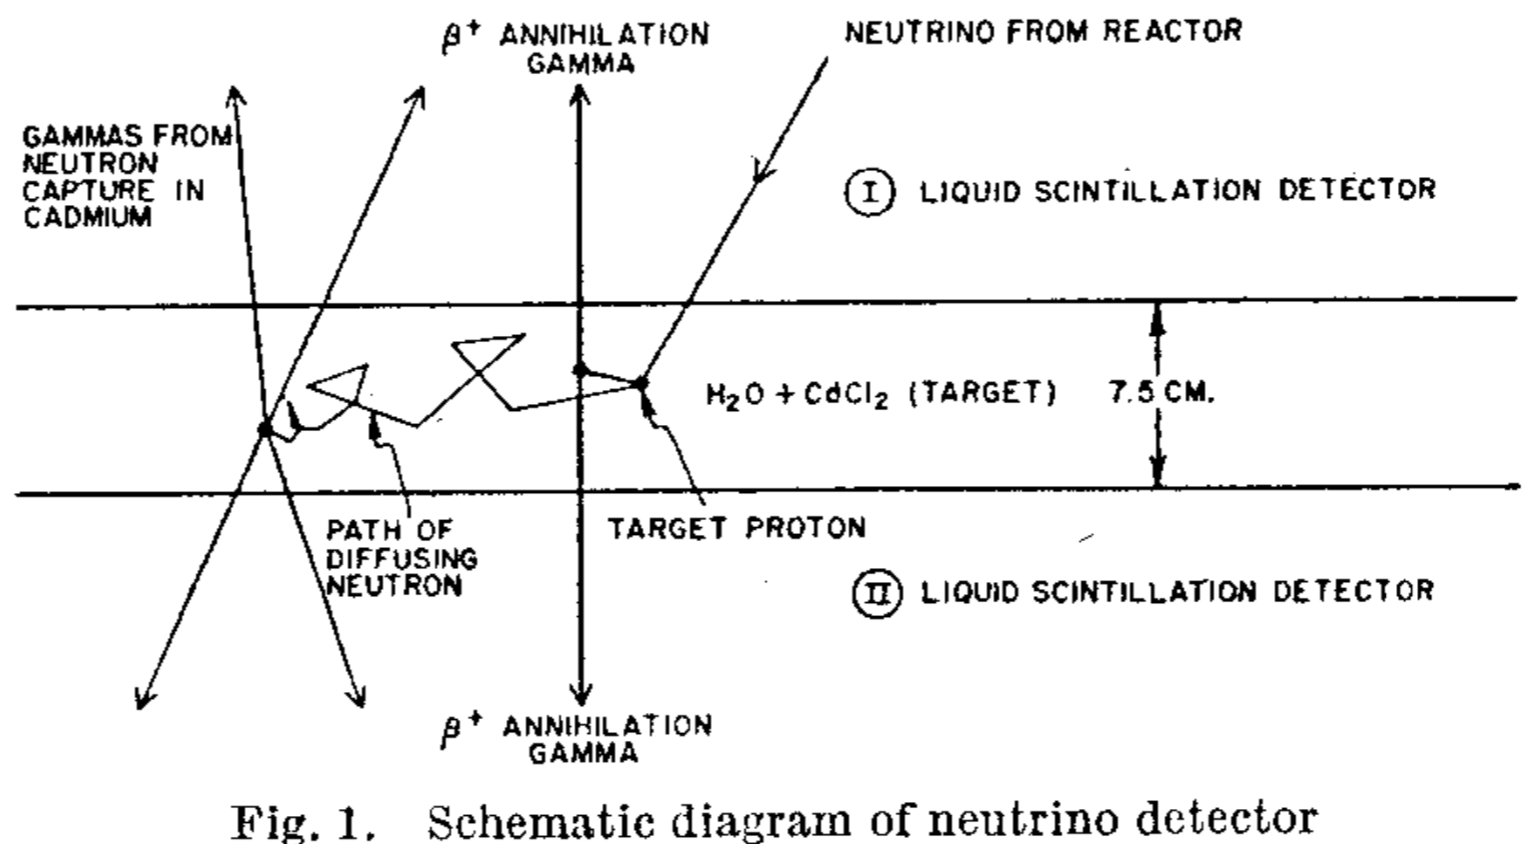
\includegraphics[width=0.75\textwidth]{imagenes/tema1/1_detector_neutrino.png}
  \caption{Esquema del dispositivo detector de neutrinos empleado por Reines y Cowan.}
  \label{fig:1_detector_neutrino}
\end{figure}

Físicamente, los dos detectores de fotones situados en coincidencia miden en primer lugar dos señales simultáneas de igual energía (señal prompt de la aniquilación del positrón), seguidas, tras un intervalo temporal característico de varios microsegundos, por un pulso de luz más intenso correspondiente a la captura neutrónica en el cadmio.

\begin{figure}[h!]
  \centering
  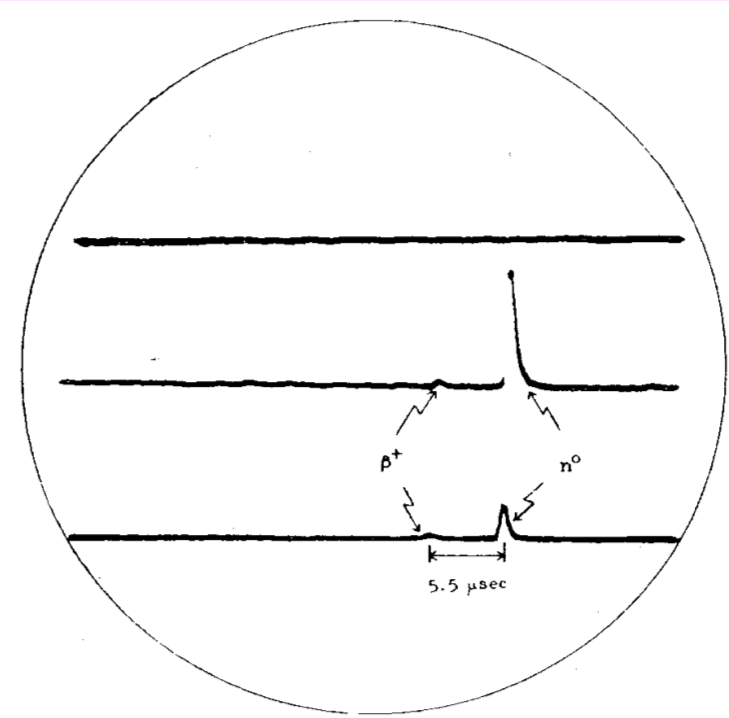
\includegraphics[width=0.75\textwidth]{imagenes/tema1/1_deteccion_neutrino.png}
  \caption{Firma temporal de la coincidencia retardada entre la aniquilación del positrón y la captura del neutrón.}
  \label{fig:1_deteccion_neutrino}
\end{figure}

\subsubsection{El Problema de los Neutrinos Solares}
Experimentos posteriores diseñados para medir el flujo de neutrinos producidos en las reacciones de fusión nuclear del Sol detectaron un número significativamente menor de neutrinos que el predicho por el Modelo Solar Estándar (problema de los neutrinos solares). La solución teórica fue propuesta por John Norris Bahcall junto con Bruno Pontecorvo, postulando que los neutrinos poseen masa finita no nula y sufren el fenómeno de \textbf{oscilación de neutrinos}, transformándose entre distintos sabores durante su trayectoria desde el núcleo solar hasta la Tierra.

\subsection{Cuestiones Fundamentales sobre la Naturaleza del Neutrino}

Una vez establecida la existencia real del neutrino, fue necesario dar respuesta a dos preguntas fundamentales sobre sus propiedades cuánticas internas.

\subsubsection{Cuestión 1: ¿Son idénticos el neutrino y el antineutrino? ($\nu \stackrel{?}{=} \bar{\nu}$)}

Para comprobar si el neutrino y el antineutrino son la misma partícula ($\nu_e = \bar{\nu}_e \equiv x_{\nu_e}$), Raymond Davis Jr. expuso un tanque de tetracloruro de carbono que contenía Cloro-37 (${}^{37}_{17}\text{Cl}$) al flujo intenso de antineutrinos producido por un reactor nuclear.

\begin{itemize}
    \item \textbf{Si $\nu_e = \bar{\nu}_e$ (Partícula de Majorana):} Deberían estar permitidas simultáneamente las dos reacciones:
    \begin{align}
    x_{\nu_e} + p &\longrightarrow n + e^+ \\
    x_{\nu_e} + n &\longrightarrow p + e^-
    \end{align}
    Por consiguiente, en el tanque de ${}^{37}_{17}\text{Cl}$ se debería observar la reacción:
    \begin{equation}
    \bar{\nu}_e + {}^{37}_{17}\text{Cl} \longrightarrow {}^{37}_{18}\text{Ar} + e^-
    \end{equation}
    
    \item \textbf{Si $\nu_e \neq \bar{\nu}_e$ (Partícula de Dirac):} La reacción $\bar{\nu}_e + n \to p + e^-$ está prohibida. En consecuencia, la transformación de ${}^{37}_{17}\text{Cl}$ en ${}^{37}_{18}\text{Ar}$ no debe producirse.
\end{itemize}

El Argón-37 (${}^{37}_{18}\text{Ar}$) es una sustancia radioactiva muy fácil de identificar al ser un emisor $\beta^+$ (captura electrónica) con un periodo de semidesintegración de $35 \text{ días}$. 

El resultado experimental de Davis fue totalmente negativo: no se midió formación de ${}^{37}_{18}\text{Ar}$. Por lo tanto, se concluye que **el neutrino y el antineutrino son partículas distintas** ($\nu_e \neq \bar{\nu}_e$). Para formalizar esta distinción se introduce la conservación del **número leptónico electrónico** ($L_e$), asignando $L_e = +1$ a $e^-$ y $\nu_e$, y $L_e = -1$ a $e^+$ y $\bar{\nu}_e$.

---

\subsubsection{Cuestión 2: ¿Existe un único tipo de neutrino para todos los leptones? ($\nu_e \stackrel{?}{=} \nu_\mu$)}

A principios de la década de 1960 se conocía la existencia del pión ($\pi^\pm$), el cual se desintegra produciendo un muón y una partícula neutra:
\begin{equation}
\pi^\pm \longrightarrow \mu^\pm + [\nu / \bar{\nu}]
\end{equation}

En 1962, L. Lederman, M. Schwartz y J. Steinberger diseñaron un experimento en Brookhaven para determinar si el neutrino asociado al muón ($\nu_\mu$) era idéntico al neutrino electrónico ($\nu_e$) emitido en la desintegración del neutrón.

\paragraph{Montaje Experimental:}
Protones de $15 \text{ GeV}$ colisionan contra un blanco de Berilio ($\text{Be}$), produciendo un haz intenso de piones $\pi^\pm$. Tras recorrer una distancia en la que los piones se desintegran ($\pi^\pm \to \mu^\pm + \nu$), el haz atraviesa un blindaje de acero de $13.5 \text{ m}$ de grosor que absorbe todos los muones y hadrones, dejando pasar únicamente a los neutrinos hacia el detector.

\paragraph{Predicción e Interpretación:}
Si $\nu_e = \nu_\mu$, los neutrinos al interaccionar con los nucleones del detector deberían producir electrones y muones en igual proporción:
\begin{align}
\bar{\nu} + p &\longrightarrow n + e^+ \qquad \text{y} \qquad \bar{\nu} + p \longrightarrow n + \mu^+ \\
\nu + n &\longrightarrow p + e^- \qquad \text{y} \qquad \nu + n \longrightarrow p + \mu^-
\end{align}

Sin embargo, en el experimento se observaron **exclusivamente eventos con muones** ($\mu^\pm$), resultando nula la producción de electrones (los escasos eventos de electrón medidos correspondían al fondo de radiación cósmica).

\paragraph{Conclusión y Ley de Conservación de Sabor Leptónico:}
Este resultado demostró que **el neutrino del muón es distinto del neutrino del electrón** ($\nu_e \neq \nu_\mu$). Cada generación de leptones posee su propio número leptónico independiente ($L_e, L_\mu, L_\tau$), cuya conservación individual prohíbe procesos de cambio de sabor sin neutrinos como:
\begin{equation}
\mu^\pm \nrightarrow e^\pm + \gamma \quad (\text{Proceso prohibido por conservación de } L_e \text{ y } L_\mu)
\end{equation}

Permitiendo únicamente la desintegración débil de los muones a través de:
\begin{align}
\mu^+ &\longrightarrow e^+ + \nu_e + \bar{\nu}_\mu \\
\mu^- &\longrightarrow e^- + \bar{\nu}_e + \nu_\mu
\end{align}















\newpage
%--------------------------------------------------------

\phantom{a}

\newpage
\section{Problemas resueltos}

% ==============================================================================
% PROBLEMA 3: UMBRAL DE PRODUCCIÓN DE ANTIPROTONES
% ==============================================================================

\begin{problema}{Problema 3}
Calcular la energía cinética mínima de un protón para que al colisionar con otro protón en reposo pueda producir antiprotones según la reacción:
\begin{equation}
p + p \longrightarrow p + p + p + \bar{p}
\end{equation}

\textit{Nota histórica:} Se trata de la reacción con la que se descubrió el antiprotón, realizada en 1955 por O. Chamberlain, E. Segrè, C. Wiegand y T. Ypsilantis.

\tcblower

\textbf{Solución:}

Para determinar la energía cinética mínima (energía umbral) necesaria en el sistema del laboratorio, emplearemos la invariancia relativista del módulo del cuadrimomento total del sistema:
\begin{equation}
s = P^\mu P_\mu = \frac{E^2}{c^2} - |\vec{p}|^2 = \text{invariante de Lorentz}
\end{equation}

---

\subsubsection*{1. Resolución en el Sistema de Referencia del Laboratorio (LAB)}

Consideramos un protón proyectil $A$ en movimiento con cuadrimomento $P_A^\mu = \left( \frac{E_A}{c}, \vec{p}_A \right)$ y un protón blanco $B$ en reposo con cuadrimomento $P_B^\mu = \left( m_p c, \vec{0} \right)$.

El cuadrimomento total del estado inicial es:
\begin{equation}
P_i^\mu = P_A^\mu + P_B^\mu = \left( \frac{E_A}{c} + m_p c, \, \vec{p}_A \right)
\end{equation}

Calculamos el invariante escalando $s$:
\begin{align}
s &= (P_i^\mu P_{i,\mu})_{\text{LAB}} = \left( \frac{E_A}{c} + m_p c \right)^2 - |\vec{p}_A|^2 \nonumber \\
  &= \frac{E_A^2}{c^2} - |\vec{p}_A|^2 + m_p^2 c^2 + 2 E_A m_p \nonumber \\
  &= m_p^2 c^2 + m_p^2 c^2 + 2 E_A m_p = 2 m_p^2 c^2 + 2 E_A m_p
\end{align}
donde se ha hecho uso de la relación relativista de dispersión $E_A^2 / c^2 - |\vec{p}_A|^2 = m_p^2 c^2$.

En la condición de umbral ($\text{th}$), las cuatro partículas del estado final ($3p + 1\bar{p}$) se producen en reposo relativo en el sistema del centro de masas ($\vec{p}_{f,\text{CM}} = \vec{0}$). Por lo tanto, la energía total mínima del estado final es la suma de sus masas en reposo:
\begin{equation}
E_{f,\text{CM}}^{\text{min}} = \sum_{i=1}^{4} m_i c^2 = 4 m_p c^2
\end{equation}

El invariante $s$ evaluado en el estado final a la energía umbral en el CM resulta:
\begin{equation}
s = (P_f^\mu P_{f,\mu})_{\text{CM}} = \left( \frac{4 m_p c^2}{c} \right)^2 = 16 m_p^2 c^2
\end{equation}

Igualando los invariantes relativistas entre el laboratorio y el centro de masas ($s_{\text{LAB}} = s_{\text{CM}}$):
\begin{equation}
2 m_p^2 c^2 + 2 E_p^{\text{LAB}} m_p = 16 m_p^2 c^2
\end{equation}
\begin{equation}
2 E_p^{\text{LAB}} m_p = 14 m_p^2 c^2 \implies E_p^{\text{LAB}} = 7 m_p c^2
\end{equation}

Por lo tanto, la energía cinética mínima (umbral) necesaria para el protón incidente en el laboratorio es:
\begin{equation}
T_p^{\text{th}} = E_p^{\text{LAB}} - m_p c^2 = 7 m_p c^2 - m_p c^2 = 6 m_p c^2
\end{equation}

Sustituyendo la masa del protón $m_p c^2 \approx 0.938 \text{ GeV}$:
\begin{equation}
T_p^{\text{th}} = 6 \times 0.938 \text{ GeV} \approx 5.63 \text{ GeV} \approx 5.6 \text{ BeV (o GeV)}
\end{equation}

---

\subsubsection*{2. Resolución en el Sistema del Centro de Masas (CM)}

En el sistema de referencia del centro de masas, ambos protones inciden con momentos iguales y opuestos:
\begin{equation}
P_A^\mu = \left( \frac{E_p^{\text{CM}}}{c}, \vec{p} \right), \qquad P_B^\mu = \left( \frac{E_p^{\text{CM}}}{c}, -\vec{p} \right)
\end{equation}

El cuadrimomento total inicial en el CM es $P_i^\mu = \left( \frac{2 E_p^{\text{CM}}}{c}, \vec{0} \right)$, cuyo invariante es:
\begin{equation}
s = (P_i^\mu P_{i,\mu})_{\text{CM}} = 4 \left( \frac{E_p^{\text{CM}}}{c} \right)^2 c^2 = 4 (E_p^{\text{CM}})^2
\end{equation}

Dado que en el umbral se crean 4 partículas idénticas de masa $m_p$ en reposo relativo, la energía total en el CM es:
\begin{equation}
E_{T}^{\text{CM}} = 2 E_p^{\text{CM}} = 4 m_p c^2 \implies E_p^{\text{CM}} = 2 m_p c^2
\end{equation}

Sustituyendo $E_p^{\text{CM}}$ en el invariante $s$:
\begin{equation}
s = 4 (2 m_p c^2)^2 = 16 m_p^2 c^2
\end{equation}

Igualando este resultado con la expresión del invariante obtenida en el laboratorio:
\begin{equation}
s_{\text{CM}} = s_{\text{LAB}} \implies 16 m_p^2 c^2 = 2 m_p^2 c^2 + 2 E_p^{\text{LAB}} m_p
\end{equation}
\begin{equation}
14 m_p^2 c^2 = 2 E_p^{\text{LAB}} m_p \implies E_p^{\text{LAB}} = 7 m_p c^2
\end{equation}

Reobteniendo así la misma energía cinética umbral $T_p^{\text{LAB}} = E_p^{\text{LAB}} - m_p c^2 = 6 m_p c^2$.

---

\subsubsection*{3. Comparación Física: Experimentos de Blanco Fijo frente a Colisionadores}

\begin{itemize}
    \item \textbf{Inconveniencia de los experimentos de blanco fijo:} Para crear una masa neta de $2 m_p c^2$ (un par protón-antiprotón $p\bar{p}$), es necesario aportar una energía cinética de $6 m_p c^2$. Las dos terceras partes de la energía introducida ($4 m_p c^2$) se pierden como energía cinética de translación del centro de masas para garantizar la conservación del momento lineal.
    \item \textbf{Ventaja de los colisionadores (ej. LHC):} En colisionadores con haces de momentos opuestos ($\vec{p}_{\text{total}} = \vec{0}$), el sistema del laboratorio coincide con el centro de masas. Toda la energía cinética de las partículas incidentes se aprovecha de forma efectiva para la producción de nuevas partículas.
    \item \textbf{Ventaja técnica del blanco fijo:} A pesar de su menor eficiencia energética, los aceleradores de blanco fijo permiten interacciones con blancos de alta densidad de materia, lo que incrementa sustancialmente la sección eficaz efectiva y la probabilidad de colisión frente a los haces cruzados.
\end{itemize}
\end{problema}

\newpage

% ==============================================================================
% PROBLEMA 4: ESTADO LIGADO DEL DEUTERÓN EN UN POZO ESFÉRICO ATRACTIVO
% ==============================================================================

\begin{problema}{Problema 4}
Suponiendo que el deuterón, sistema formado por un neutrón y un protón, se pudiera describir como un estado ligado en onda $S$ ($L=0$), dar una estimación de la profundidad del pozo para un potencial de la forma:
\begin{equation}
V(r) = \begin{cases} -V_0, & r \le a \\ 0, & r > a \end{cases}
\end{equation}
siendo $a = 1.59 \text{ fm}$. Considerar que la energía de ligadura, $B = -E$, es mucho menor que la profundidad del pozo, $V_0$. 

Representar gráficamente el comportamiento de la función de onda reducida, $u_L(r)$, que satisface la ecuación:
\begin{equation}
\left( -\frac{\hbar^2}{2\mu} \frac{d^2}{dr^2} + V(r) + \frac{\hbar^2 L(L+1)}{2\mu r^2} \right) u_L(r) = E u_L(r)
\end{equation}

\tcblower

\textbf{Solución:}

\subsubsection*{1. Separación de Variables y Ecuación Radial Reducida}

Para un estado de momento angular orbital nulo ($L = 0$, onda $S$), el armónico esférico correspondiente es constante:
\begin{equation}
Y_{00}(\Omega) = \frac{1}{\sqrt{4\pi}} \implies \psi(\vec{r}) = R(r) Y_{00}(\Omega) = \frac{u(r)}{r} Y_{00}(\Omega)
\end{equation}

donde $R(r) = \frac{u(r)}{r}$ representa la función de onda radial y $u(r)$ es la función radial reducida. La ecuación de Schrödinger radial completa se reduce a:
\begin{equation}
\left( -\frac{\hbar^2}{2\mu} \frac{d^2}{dr^2} + V(r) + \frac{\hbar^2 L(L+1)}{2\mu r^2} \right) u(r) = E u(r)
\end{equation}

Al ser $L = 0$, el término de la barrera centrífuga se anula, resultando la ecuación diferencial unidimensional:
\begin{equation}
\frac{d^2 u(r)}{dr^2} + \frac{2\mu}{\hbar^2} \left( E - V(r) \right) u(r) = 0
\end{equation}

---

\subsubsection*{2. Solución en las Regiones del Potencial}

Analizamos la solución general en las dos regiones de continuidad del potencial de pozo cuadrado esférico para un estado ligado ($E = -B < 0$, con $B > 0$):

\paragraph{Zona I ($r \le a$, $V(r) = -V_0$):}
En el interior del pozo, el potencial es constante y atractivo:
\begin{equation}
\frac{d^2 u_I(r)}{dr^2} + \frac{2\mu}{\hbar^2} (V_0 - B) u_I(r) = 0 \implies \frac{d^2 u_I(r)}{dr^2} + \alpha^2 u_I(r) = 0
\end{equation}
donde definimos la constante de onda interna $\alpha$:
\begin{equation}
\alpha = \frac{\sqrt{2\mu (V_0 - B)}}{\hbar} = \frac{\sqrt{2\mu (V_0 + E)}}{\hbar}
\end{equation}

La solución general de esta ecuación armónica es:
\begin{equation}
u_I(r) = A \sin(\alpha r) + B' \cos(\alpha r)
\end{equation}

Para garantizar la regularidad de la función de onda en el origen ($r = 0$), se exige la condición de contorno $R(0) < \infty \implies u(0) = 0$. Dado que $\cos(0) = 1$, la constante $B'$ debe ser nula ($B' = 0$), quedando:
\begin{equation}
u_I(r) = A \sin(\alpha r)
\end{equation}

\paragraph{Zona II ($r > a$, $V(r) = 0$):}
Fuera del pozo, la partícula se encuentra en la región clásicamente prohibida:
\begin{equation}
\frac{d^2 u_{II}(r)}{dr^2} - \frac{2\mu B}{\hbar^2} u_{II}(r) = 0 \implies \frac{d^2 u_{II}(r)}{dr^2} - k^2 u_{II}(r) = 0
\end{equation}
donde definimos la constante de atenuación externa $k$:
\begin{equation}
k = \frac{\sqrt{2\mu B}}{\hbar} = \frac{\sqrt{-2\mu E}}{\hbar}
\end{equation}

La solución general es una combinación de exponenciales real e invertida:
\begin{equation}
u_{II}(r) = C e^{-k r} + C' e^{+k r}
\end{equation}

Para que la función de onda sea normalizable y tienda a cero en el infinito ($u_{II}(r) \to 0$ cuando $r \to \infty$), se requiere $C' = 0$, obteniendo:
\begin{equation}
u_{II}(r) = C e^{-k r}
\end{equation}

---

\subsubsection*{3. Condiciones de Contorno e Igualdad de la Derivada Logarítmica}

Para garantizar la continuidad de la función de onda $u(r)$ y de su primera derivada $u'(r)$ en la frontera $r = a$, igualamos la derivada logarítmica a ambos lados:
\begin{equation}
\left. \frac{u_I'(r)}{u_I(r)} \right|_{r=a} = \left. \frac{u_{II}'(r)}{u_{II}(r)} \right|_{r=a}
\end{equation}

Sustituyendo $u_I(r) = A \sin(\alpha r)$ y $u_{II}(r) = C e^{-k r}$:
\begin{equation}
\frac{A \alpha \cos(\alpha a)}{A \sin(\alpha a)} = \frac{-C k e^{-k a}}{C e^{-k a}} \implies \alpha \cot(\alpha a) = -k
\end{equation}

Reagrupando la condición trascendente de cuantización:
\begin{equation}
\tan(\alpha a) = -\frac{\alpha}{k}
\end{equation}

---

\subsubsection*{4. Condición de Pozo Poco Ligado ($V_0 \gg B$)}

Utilizando el enunciado, sabemos que el deuterón es un sistema débilmente ligado donde la energía de ligadura $B = -E$ es mucho menor que la profundidad del pozo $V_0$ ($V_0 \gg B$):
\begin{equation}
\frac{\alpha}{k} = \frac{\sqrt{2\mu(V_0 - B)}/\hbar}{\sqrt{2\mu B}/\hbar} = \sqrt{\frac{V_0 - B}{B}} \approx \sqrt{\frac{V_0}{B}} \gg 1
\end{equation}

Puesto que el cociente $\frac{\alpha}{k}$ es un valor numérico muy grande, el término $-\frac{\alpha}{k}$ tiende a $-\infty$. Para que la función tangente tienda a $-\infty$, su argumento debe aproximarse por la izquierda al primer polo ($\pi / 2$) correspondiente al primer estado ligado (estado fundamental):
\begin{equation}
\alpha a \approx \frac{\pi}{2}
\end{equation}

---

\subsubsection*{5. Representación Gráfica de la Función de Onda Reducida $u(r)$}

\begin{center}
\begin{tikzpicture}[scale=1.1]
  % Ejes coordenados
  \draw[->, thick] (0,0) -- (6.0,0) node[right] {$r$};
  \draw[->, thick] (0,-1.8) -- (0,2.8) node[above] {$u(r), V(r)$};
  
  % Pozo de potencial esquematico
  \draw[dashed, red!80!black, thick] (0,-1.2) -- (2.2,-1.2) -- (2.2,0) -- (5.5,0);
  \node[red!80!black, left] at (0,-1.2) {$-V_0$};
  \node[red!80!black, above] at (1.1,-1.2) {$V(r) = -V_0$};
  
  % Línea del radio del pozo
  \draw[dotted, gray, thick] (2.2,-1.5) -- (2.2,2.3);
  \node[below, black] at (2.2,0) {$r = a$};
  
  % Region I: Curva senoidal u_I(r)
  \draw[domain=0:2.2, samples=100, smooth, ultra thick, maincolor] 
    plot (\x, {2.2*sin(deg(\x * 3.14159 / (2*2.2)))});
    
  % Region II: Curva exponencial decreciente u_II(r)
  \draw[domain=2.2:5.5, samples=100, smooth, ultra thick, maincolor] 
    plot (\x, {2.2*exp(-0.85*(\x - 2.2))});
    
  % Etiquetas de las soluciones
  \node[maincolor, above] at (1.1,1.5) {$u_I(r) = A \sin(\alpha r)$};
  \node[maincolor, above right] at (3.0,1.0) {$u_{II}(r) = C e^{-kr}$};
  
  % Punto de empalme suave
  \fill[maincolor] (2.2,2.2) circle (2pt);
  \node[above] at (2.2,2.3) {\small Empalme C$^1$ en $r=a$};
\end{tikzpicture}
\end{center}
\end{problema}

\newpage

% ==============================================================================
% EJERCICIO 12: ACOPLAMIENTO DE MOMENTOS ANGULARES Y SIMETRÍA DE ESPÍN
% Solución completa: Apartado a) operadores de escalera y Clebsch-Gordan;
% Apartado b) desarrollo explícito de la simetría de espín para s_a = 0, 1/2, 1
% ==============================================================================

\begin{problema}{Ejercicio 12}
\begin{enumerate}[label=\alph*)]
    \item El momento angular orbital $\ell$ y el espín de un electrón en un átomo de hidrógeno pueden acoplarse para dar dos valores del momento angular total $j = \ell \pm \frac{1}{2}$. Así, los estados P ($\ell = 1$) pueden tener $j = \frac{3}{2}$ (tetraplete) ó $j = \frac{1}{2}$ (doblete). 
    
    El estado $|j, m\rangle = \left|\frac{3}{2}, \frac{3}{2}\right\rangle$ viene definido unívocamente por el estado $|\ell, m_\ell\rangle \otimes |s, m_s\rangle = |1, 1\rangle \otimes \left|\frac{1}{2}, \frac{1}{2}\right\rangle$. Utilizar los operadores $J_- = L_- + S_-$ para obtener los otros tres estados del tetraplete. Comprobar la solución con la obtenida utilizando tablas de coeficientes de Clebsch-Gordan.

    \textit{Nota:} La actuación de los operadores de escalera $J_\pm$ sobre un estado genérico $|j, m\rangle$ viene dada por:
    \begin{equation}
    J_\pm |j, m\rangle = \sqrt{j(j+1) - m(m \pm 1)} \, |j, m \pm 1\rangle
    \end{equation}

    \item Considerar dos partículas idénticas de espín $s_a$. Determinar la simetría de la función de onda de espín total en los casos: $s_a = 0$, $s_a = 1/2$ y $s_a = 1$.
\end{enumerate}

\tcblower

\textbf{Solución:}

\subsubsection*{Apartado a) Obtención de los estados del tetraplete mediante operadores de descenso}

Trabajamos con el acoplamiento de un momento angular orbital $\ell = 1$ y un espín $s = 1/2$. El tetraplete corresponde al valor de momento angular total $j = 3/2$, con proyecciones $m_j \in \{+3/2, +1/2, -1/2, -3/2\}$.

Para simplificar la notación, denotaremos la base desacoplada $|\ell, m_\ell\rangle |s, m_s\rangle$ simplemente como $|m_\ell\rangle |m_s\rangle$.

\paragraph{1. Estado de máxima proyección ($m_j = +3/2$):}
El estado superior del tetraplete es único y coincide exactamente con el producto directo de los estados de máxima proyección orbital y de espín:
\begin{equation}
\left| \frac{3}{2}, \frac{3}{2} \right\rangle = |1, 1\rangle \left| \frac{1}{2}, \frac{1}{2} \right\rangle
\end{equation}

\paragraph{2. Obtención del estado $\left| \frac{3}{2}, \frac{1}{2} \right\rangle$:}
Aplicamos el operador de descenso $J_- = L_- + S_-$ a ambos lados de la igualdad anterior.

\textit{Lado izquierdo (base acoplada):}
\begin{align}
J_- \left| \frac{3}{2}, \frac{3}{2} \right\rangle &= \sqrt{\frac{3}{2}\left(\frac{3}{2}+1\right) - \frac{3}{2}\left(\frac{3}{2}-1\right)} \left| \frac{3}{2}, \frac{1}{2} \right\rangle \nonumber \\
&= \sqrt{\frac{15}{4} - \frac{3}{4}} \left| \frac{3}{2}, \frac{1}{2} \right\rangle = \sqrt{3} \left| \frac{3}{2}, \frac{1}{2} \right\rangle
\end{align}

\textit{Lado derecho (base desacoplada):}
\begin{align}
(L_- + S_-) \left[ |1, 1\rangle \left| \frac{1}{2}, \frac{1}{2} \right\rangle \right] &= (L_- |1, 1\rangle) \left| \frac{1}{2}, \frac{1}{2} \right\rangle + |1, 1\rangle \left( S_- \left| \frac{1}{2}, \frac{1}{2} \right\rangle \right) \nonumber \\
&= \sqrt{1(1+1) - 1(0)} \, |1, 0\rangle \left| \frac{1}{2}, \frac{1}{2} \right\rangle + |1, 1\rangle \sqrt{\frac{1}{2}\left(\frac{3}{2}\right) - \frac{1}{2}\left(-\frac{1}{2}\right)} \left| \frac{1}{2}, -\frac{1}{2} \right\rangle \nonumber \\
&= \sqrt{2} \, |1, 0\rangle \left| \frac{1}{2}, \frac{1}{2} \right\rangle + |1, 1\rangle \left| \frac{1}{2}, -\frac{1}{2} \right\rangle
\end{align}

Igualando ambas expresiones y despejando $\left| \frac{3}{2}, \frac{1}{2} \right\rangle$:
\begin{equation}
\left| \frac{3}{2}, \frac{1}{2} \right\rangle = \sqrt{\frac{2}{3}} \, |1, 0\rangle \left| \frac{1}{2}, \frac{1}{2} \right\rangle + \sqrt{\frac{1}{3}} \, |1, 1\rangle \left| \frac{1}{2}, -\frac{1}{2} \right\rangle
\end{equation}

\paragraph{3. Obtención del estado $\left| \frac{3}{2}, -\frac{1}{2} \right\rangle$:}
Aplicamos nuevamente $J_-$ sobre el estado obtenido en el paso anterior.

\textit{Lado izquierdo:}
\begin{equation}
J_- \left| \frac{3}{2}, \frac{1}{2} \right\rangle = \sqrt{\frac{3}{2}\left(\frac{5}{2}\right) - \frac{1}{2}\left(-\frac{1}{2}\right)} \left| \frac{3}{2}, -\frac{1}{2} \right\rangle = \sqrt{\frac{15}{4} + \frac{1}{4}} \left| \frac{3}{2}, -\frac{1}{2} \right\rangle = 2 \left| \frac{3}{2}, -\frac{1}{2} \right\rangle
\end{equation}

\textit{Lado derecho:}
\begin{align}
(L_- + S_-) &\left[ \sqrt{\frac{2}{3}} |1, 0\rangle \left| \frac{1}{2}, \frac{1}{2} \right\rangle + \sqrt{\frac{1}{3}} |1, 1\rangle \left| \frac{1}{2}, -\frac{1}{2} \right\rangle \right] \nonumber \\
&= \sqrt{\frac{2}{3}} \left[ \sqrt{2} |1, -1\rangle \left| \frac{1}{2}, \frac{1}{2} \right\rangle + |1, 0\rangle \left| \frac{1}{2}, -\frac{1}{2} \right\rangle \right] + \sqrt{\frac{1}{3}} \left[ \sqrt{2} |1, 0\rangle \left| \frac{1}{2}, -\frac{1}{2} \right\rangle + 0 \right] \nonumber \\
&= \frac{2}{\sqrt{3}} |1, -1\rangle \left| \frac{1}{2}, \frac{1}{2} \right\rangle + \left( \sqrt{\frac{2}{3}} + \frac{\sqrt{2}}{\sqrt{3}} \right) |1, 0\rangle \left| \frac{1}{2}, -\frac{1}{2} \right\rangle \nonumber \\
&= \frac{2}{\sqrt{3}} |1, -1\rangle \left| \frac{1}{2}, \frac{1}{2} \right\rangle + 2 \sqrt{\frac{2}{3}} |1, 0\rangle \left| \frac{1}{2}, -\frac{1}{2} \right\rangle
\end{align}

Dividiendo entre $2$ a ambos lados:
\begin{equation}
\left| \frac{3}{2}, -\frac{1}{2} \right\rangle = \sqrt{\frac{1}{3}} \, |1, -1\rangle \left| \frac{1}{2}, \frac{1}{2} \right\rangle + \sqrt{\frac{2}{3}} \, |1, 0\rangle \left| \frac{1}{2}, -\frac{1}{2} \right\rangle
\end{equation}

\paragraph{4. Obtención del estado $\left| \frac{3}{2}, -\frac{3}{2} \right\rangle$:}
Aplicamos $J_-$ por tercera vez.

\textit{Lado izquierdo:}
\begin{equation}
J_- \left| \frac{3}{2}, -\frac{1}{2} \right\rangle = \sqrt{\frac{15}{4} - \left(-\frac{1}{2}\right)\left(-\frac{3}{2}\right)} \left| \frac{3}{2}, -\frac{3}{2} \right\rangle = \sqrt{3} \left| \frac{3}{2}, -\frac{3}{2} \right\rangle
\end{equation}

\textit{Lado derecho:}
\begin{align}
(L_- + S_-) &\left[ \sqrt{\frac{1}{3}} |1, -1\rangle \left| \frac{1}{2}, \frac{1}{2} \right\rangle + \sqrt{\frac{2}{3}} |1, 0\rangle \left| \frac{1}{2}, -\frac{1}{2} \right\rangle \right] \nonumber \\
&= \sqrt{\frac{1}{3}} \left[ 0 + |1, -1\rangle \left| \frac{1}{2}, -\frac{1}{2} \right\rangle \right] + \sqrt{\frac{2}{3}} \left[ \sqrt{2} |1, -1\rangle \left| \frac{1}{2}, -\frac{1}{2} \right\rangle + 0 \right] \nonumber \\
&= \left( \frac{1}{\sqrt{3}} + \frac{2}{\sqrt{3}} \right) |1, -1\rangle \left| \frac{1}{2}, -\frac{1}{2} \right\rangle = \frac{3}{\sqrt{3}} |1, -1\rangle \left| \frac{1}{2}, -\frac{1}{2} \right\rangle = \sqrt{3} \, |1, -1\rangle \left| \frac{1}{2}, -\frac{1}{2} \right\rangle
\end{align}

Dividiendo entre $\sqrt{3}$:
\begin{equation}
\left| \frac{3}{2}, -\frac{3}{2} \right\rangle = |1, -1\rangle \left| \frac{1}{2}, -\frac{1}{2} \right\rangle
\end{equation}

\paragraph{Comprobación con Coeficientes de Clebsch-Gordan:}
La relación general de cambio de base viene dada por los coeficientes de Clebsch-Gordan:
\begin{equation}
|j, m_j\rangle = \sum_{m_{\ell}, m_s} \langle \ell, s; m_\ell, m_s | j, m_j \rangle \, |\ell, m_\ell\rangle |s, m_s\rangle
\end{equation}
Consultando la tabla de acoplamiento $1 \otimes 1/2$:
\begin{itemize}
    \item Para $j = 3/2, m_j = 3/2$: $\langle 1, 1/2; 1, 1/2 | 3/2, 3/2 \rangle = 1$.
    \item Para $j = 3/2, m_j = 1/2$: $\langle 1, 1/2; 0, 1/2 | 3/2, 1/2 \rangle = \sqrt{2/3}$, \quad $\langle 1, 1/2; 1, -1/2 | 3/2, 1/2 \rangle = \sqrt{1/3}$.
    \item Para $j = 3/2, m_j = -1/2$: $\langle 1, 1/2; -1, 1/2 | 3/2, -1/2 \rangle = \sqrt{1/3}$, \quad $\langle 1, 1/2; 0, -1/2 | 3/2, -1/2 \rangle = \sqrt{2/3}$.
    \item Para $j = 3/2, m_j = -3/2$: $\langle 1, 1/2; -1, -1/2 | 3/2, -3/2 \rangle = 1$.
\end{itemize}
Los coeficientes obtenidos mediante los operadores de escalera coinciden exactamente con los de la tabla.

\subsubsection*{Apartado b) Desarrollo completo y clasificación de simetría para $s_a = 0$, $s_a = 1/2$ y $s_a = 1$}

El operador de permutación $P_{12}$ intercambia las etiquetas de dos partículas idénticas. Para dos partículas de espín $s_a$ acopladas a un espín total $S \in \{2s_a, 2s_a - 1, \dots, 0\}$, la acción de $P_{12}$ sobre un estado de la base acoplada $|S, M_S\rangle$ satisface la propiedad general:
\begin{equation}
P_{12} |S, M_S\rangle = (-1)^{2s_a - S} |S, M_S\rangle
\end{equation}
A continuación se realiza la construcción explícita de las combinaciones lineales en la base desacoplada y la verificación de su simetría bajo el intercambio de las dos partículas ($1 \leftrightarrow 2$) para los tres casos propuestos.

\paragraph{1. Caso $s_a = 0$ (Bosones escalar / sin espín):}
El acoplamiento de dos partículas con $s_1 = 0$ y $s_2 = 0$ conduce a un único valor posible de espín total:
\begin{equation}
0 \otimes 0 \implies S = 0 \quad (\text{dim: } 1 \times 1 = 1 \text{ estado})
\end{equation}

El estado resultante es el singlete $|0, 0\rangle = |0, 0\rangle_1 |0, 0\rangle_2$. Bajo el operador de permutación:
\begin{equation}
P_{12} |0, 0\rangle = (-1)^{2(0) - 0} |0, 0\rangle = +1 |0, 0\rangle \quad (\mathbf{\text{Simétrico}})
\end{equation}

\paragraph{2. Caso $s_a = 1/2$ (Fermiones de espín $1/2$):}
El acoplamiento de dos fermiones de espín $s_1 = 1/2$ y $s_2 = 1/2$ genera:
\begin{equation}
\frac{1}{2} \otimes \frac{1}{2} \implies S = 1 \oplus 0 \quad (\text{dim: } 2 \times 2 = 4 \text{ estados})
\end{equation}

\subparagraph{A. Triplete de Espín ($S = 1$, 3 estados):}
Partiendo de los estados de máxima y mínima proyección $M_S = \pm 1$:
\begin{align}
|1, 1\rangle &= \left|\frac{1}{2}, \frac{1}{2}\right\rangle_1 \left|\frac{1}{2}, \frac{1}{2}\right\rangle_2 \quad \xrightarrow{P_{12}} \quad +|1, 1\rangle \quad (\mathbf{\text{Simétrico}}) \\
|1, -1\rangle &= \left|\frac{1}{2}, -\frac{1}{2}\right\rangle_1 \left|\frac{1}{2}, -\frac{1}{2}\right\rangle_2 \quad \xrightarrow{P_{12}} \quad +|1, -1\rangle \quad (\mathbf{\text{Simétrico}})
\end{align}

Para la proyección $M_S = 0$, utilizando la tabla de coeficientes de Clebsch-Gordan o aplicando el operador de descenso $S_- = S_{1,-} + S_{2,-}$:
\begin{equation}
|1, 0\rangle = \frac{1}{\sqrt{2}} \left|\frac{1}{2}, \frac{1}{2}\right\rangle_1 \left|\frac{1}{2}, -\frac{1}{2}\right\rangle_2 + \frac{1}{\sqrt{2}} \left|\frac{1}{2}, -\frac{1}{2}\right\rangle_1 \left|\frac{1}{2}, \frac{1}{2}\right\rangle_2
\end{equation}
Al intercambiar los índices $1 \leftrightarrow 2$, el estado permanece inalterado: $P_{12} |1, 0\rangle = +|1, 0\rangle$ ($\mathbf{\text{Simétrico}}$).

\subparagraph{B. Singlete de Espín ($S = 0$, 1 estado):}
El estado ortogonal con proyección $M_S = 0$ es:
\begin{equation}
|0, 0\rangle = \frac{1}{\sqrt{2}} \left|\frac{1}{2}, \frac{1}{2}\right\rangle_1 \left|\frac{1}{2}, -\frac{1}{2}\right\rangle_2 - \frac{1}{\sqrt{2}} \left|\frac{1}{2}, -\frac{1}{2}\right\rangle_1 \left|\frac{1}{2}, \frac{1}{2}\right\rangle_2
\end{equation}
Al intercambiar los índices $1 \leftrightarrow 2$, la función cambia de signo global: $P_{12} |0, 0\rangle = -|0, 0\rangle$ ($\mathbf{\text{Antisimétrico}}$).

\textbf{Resumen para $s_a = 1/2$:}
\begin{itemize}
    \item $S = 1$ (3 estados): Factor $(-1)^{2(1/2) - 1} = (-1)^0 = +1 \implies \mathbf{3 \text{ estados simétricos}}$.
    \item $S = 0$ (1 estado): Factor $(-1)^{2(1/2) - 0} = (-1)^1 = -1 \implies \mathbf{1 \text{ estado antisimétrico}}$.
\end{itemize}

\paragraph{3. Caso $s_a = 1$ (Bosones de espín $1$):}
El acoplamiento de dos bosones vectoriales $s_1 = 1$ y $s_2 = 1$ genera:
\begin{equation}
1 \otimes 1 \implies S = 2 \oplus 1 \oplus 0 \quad (\text{dim: } 3 \times 3 = 9 \text{ estados})
\end{equation}

\subparagraph{A. Quintuplete de Espín ($S = 2$, 5 estados):}
Los estados de proyección extrema son directamente simétricos:
\begin{align}
|2, 2\rangle &= |1, 1\rangle_1 |1, 1\rangle_2 \quad (\mathbf{\text{Simétrico}}) \\
|2, -2\rangle &= |1, -1\rangle_1 |1, -1\rangle_2 \quad (\mathbf{\text{Simétrico}})
\end{align}

Obteniendo los estados restantes mediante el operador de descenso o los coeficientes de Clebsch-Gordan $1 \otimes 1$:
\begin{align}
|2, 1\rangle &= \frac{1}{\sqrt{2}} |1, 1\rangle_1 |1, 0\rangle_2 + \frac{1}{\sqrt{2}} |1, 0\rangle_1 |1, 1\rangle_2 \quad (\mathbf{\text{Simétrico}}) \\
|2, 0\rangle &= \frac{1}{\sqrt{6}} |1, 1\rangle_1 |1, -1\rangle_2 + \sqrt{\frac{2}{3}} |1, 0\rangle_1 |1, 0\rangle_2 + \frac{1}{\sqrt{6}} |1, -1\rangle_1 |1, 1\rangle_2 \quad (\mathbf{\text{Simétrico}}) \\
|2, -1\rangle &= \frac{1}{\sqrt{2}} |1, 0\rangle_1 |1, -1\rangle_2 + \frac{1}{\sqrt{2}} |1, -1\rangle_1 |1, 0\rangle_2 \quad (\mathbf{\text{Simétrico}})
\end{align}
Los 5 estados del multiplete $S = 2$ son estrictamente \textbf{simétricos} bajo el operador $P_{12}$.

\subparagraph{B. Triplete de Espín ($S = 1$, 3 estados):}
Los estados ortogonales con $S = 1$ se construyen como diferencias antisimétricas:
\begin{align}
|1, 1\rangle &= \frac{1}{\sqrt{2}} |1, 1\rangle_1 |1, 0\rangle_2 - \frac{1}{\sqrt{2}} |1, 0\rangle_1 |1, 1\rangle_2 \quad (\mathbf{\text{Antisimétrico}}) \\
|1, 0\rangle &= \frac{1}{\sqrt{2}} |1, 1\rangle_1 |1, -1\rangle_2 - \frac{1}{\sqrt{2}} |1, -1\rangle_1 |1, 1\rangle_2 \quad (\mathbf{\text{Antisimétrico}}) \\
|1, -1\rangle &= \frac{1}{\sqrt{2}} |1, 0\rangle_1 |1, -1\rangle_2 - \frac{1}{\sqrt{2}} |1, -1\rangle_1 |1, 0\rangle_2 \quad (\mathbf{\text{Antisimétrico}})
\end{align}
Los 3 estados del multiplete $S = 1$ son estrictamente \textbf{antisimétricos} bajo el operador $P_{12}$.

\subparagraph{C. Singlete de Espín ($S = 0$, 1 estado):}
El estado totalmente ortogonal para $S = 0$ adopta la forma:
\begin{equation}
|0, 0\rangle = \frac{1}{\sqrt{3}} |1, 1\rangle_1 |1, -1\rangle_2 - \frac{1}{\sqrt{3}} |1, 0\rangle_1 |1, 0\rangle_2 + \frac{1}{\sqrt{3}} |1, -1\rangle_1 |1, 1\rangle_2
\end{equation}
Al permutar las partículas $1 \leftrightarrow 2$, el primer y tercer término se transforman mutuamente mientras el término central permanece idéntico, resultando $P_{12} |0, 0\rangle = +|0, 0\rangle$ ($\mathbf{\text{Simétrico}}$).

\textbf{Resumen para $s_a = 1$:}
\begin{itemize}
    \item $S = 2$ (5 estados): Factor $(-1)^{2(1) - 2} = (-1)^0 = +1 \implies \mathbf{5 \text{ estados simétricos}}$.
    \item $S = 1$ (3 estados): Factor $(-1)^{2(1) - 1} = (-1)^1 = -1 \implies \mathbf{3 \text{ estados antisimétricos}}$.
    \item $S = 0$ (1 estado): Factor $(-1)^{2(1) - 0} = (-1)^2 = +1 \implies \mathbf{1 \text{ estado simétrico}}$.
\end{itemize}

Para dos bosones de dimensión individual $N = 2s_a + 1 = 3$, el número total de estados simétricos es $\frac{N(N+1)}{2} = \frac{3 \times 4}{2} = 6$ ($5 + 1$), y el de estados antisimétricos es $\frac{N(N-1)}{2} = \frac{3 \times 2}{2} = 3$.

\paragraph{Conclusión general de simetría:}
Los resultados anteriores para $s_a = 0, 1/2, 1$ ponen de manifiesto una regla general que depende únicamente de la naturaleza cuántica (fermiónica o bosónica) de las dos partículas idénticas acopladas:
\begin{itemize}
    \item \textbf{Fermiones} (espín semientero $s_a$): si se acoplan a un momento angular total $S$ \textbf{impar}, el estado de espín resultante es \textbf{simétrico}; si $S$ es \textbf{par}, el estado es \textbf{antisimétrico}.
    \item \textbf{Bosones} (espín entero $s_a$): la regla es exactamente la inversa. Si $S$ es \textbf{par}, el estado es \textbf{simétrico}; si $S$ es \textbf{impar}, el estado es \textbf{antisimétrico}.
\end{itemize}
Esta regla se deduce directamente del factor de fase $(-1)^{2s_a - S}$: para fermiones $2s_a$ es impar, por lo que el signo global resulta $+1$ cuando $S$ es impar y $-1$ cuando $S$ es par; para bosones $2s_a$ es par, y el signo sigue entonces la paridad de $S$ de forma directa, invirtiendo así el criterio respecto al caso fermiónico.
\end{problema}

% \input{tema2.tex}
% \input{tema3.tex}
% \input{tema4.tex}

%% !TEX root = ../main.tex

\chapter{Problemas Adicionales}
\label{chap:problemas_adicionales}

% ==============================================================================
% SECCIÓN 1: BÁSICOS
% ==============================================================================

\section{Problemas básicos}

\subsection*{1. Masa Nuclear, Defecto de Masa y Energía de Ligadura}

La masa de un átomo neutro $M(Z,A)$ constituido por $Z$ protones y $N = A - Z$ neutrones es siempre inferior a la suma de las masas de sus nucleones componentes libres ($Z$ átomos de hidrógeno ${}^1\text{H}$ y $N$ neutrones $n$):
\begin{equation}
M(Z,A) < Z M({}^1\text{H}) + N m_n
\end{equation}

Esta diferencia de masa se denomina \textbf{defecto de masa} ($\Delta M$) y representa la energía liberada durante la formación del estado ligado nuclear:
\begin{equation}
\Delta M(Z,A) \equiv Z M({}^1\text{H}) + N m_n - M(Z,A)
\end{equation}

La \textbf{energía de ligadura} ($B$) es la energía mínima necesaria para disgregar completamente un núcleo en sus nucleones constitutivos individuales:
\begin{equation}
B(Z,A) = \Delta M(Z,A) c^2 = \left[ Z M({}^1\text{H}) + (A - Z) m_n - M(Z,A) \right] c^2
\end{equation}

En la práctica, las masas atómicas se expresan en unidades de masa atómica ($\text{u}$), donde $1\text{ u} \equiv 1/12 \, M({}^{12}\text{C}) \approx 931.5\text{ MeV}/c^2$. La estabilidad relativa entre diferentes núcleos se mide mediante la \textbf{energía de ligadura por nucleón} ($B/A$), la cual alcanza un máximo de aproximadamente $8.7\text{ MeV/nucleón}$ en la región del hierro ($A \approx 56$).

\subsection*{2. Distribuciones de Carga, Factor de Forma y Energía Culombiana}

\subsubsection*{2.1. Factor de forma y radio cuadrático medio}
La distribución espacial de la carga nuclear $\rho(\vec{r})$ determina la desviación de la dispersión de electrones respecto a la dispersión puntual de Rutherford. El \textbf{factor de forma electromagnético} $G(q^2)$ es la transformada de Fourier de la densidad de carga:
\begin{equation}
G(q^2) = \int \rho(\vec{r}) e^{i \vec{q} \cdot \vec{r} / \hbar} d^3r
\end{equation}

Para transferencias de momento pequeñas ($q^2 \to 0$), el desarrollo en serie del factor de forma relaciona directamente su pendiente con el \textbf{radio cuadrático medio} $\langle r^2 \rangle$:
\begin{equation}
G(q^2) = 1 - \frac{1}{6\hbar^2} \langle r^2 \rangle q^2 + \mathcal{O}(q^4) \implies \langle r^2 \rangle = -6\hbar^2 \left. \frac{d G(q^2)}{d(q^2)} \right|_{q^2=0}
\end{equation}

\subsubsection*{2.2. Energía de repulsión de Coulomb}
La repulsión electrostática entre los protones genera una energía potencial de Coulomb $U_c$ que reduce la ligadura del núcleo ($B = B_{\text{fuerte}} - U_c$). Para una carga total $Q = Z e$ repartida en una esfera de radio $R$:
\begin{itemize}
    \item \textbf{Distribución volumétrica homogénea:}
    \begin{equation}
    U_c(\text{vol}) = \frac{3}{5} \frac{1}{4\pi\varepsilon_0} \frac{Z(Z-1) e^2}{R}
    \end{equation}
    \item \textbf{Distribución superficial pura:}
    \begin{equation}
    U_c(\text{sup}) = \frac{1}{2} \frac{1}{4\pi\varepsilon_0} \frac{Z(Z-1) e^2}{R}
    \end{equation}
\end{itemize}

El cociente entre ambas configuraciones es constante:
\begin{equation}
\frac{U_c(\text{vol})}{U_c(\text{sup})} = \frac{3/5}{1/2} = \frac{6}{5} = 1.2
\end{equation}

En los \textbf{isóbaros espejo} ($Z_1 = Z, N_1 = Z-1$ frente a $Z_2 = Z-1, N_2 = Z$), la interacción fuerte es idéntica ($V_{pp} \approx V_{nn}$). Por ello, la diferencia entre sus energías de ligadura permite determinar experimentalmente el radio nuclear común $R$:
\begin{equation}
\Delta B = B(Z-1, A) - B(Z, A) = U_c(Z) - U_c(Z-1) = \frac{3}{5} \frac{e^2}{4\pi\varepsilon_0 R} \left[ Z(Z-1) - (Z-1)(Z-2) \right]
\end{equation}

\subsection*{3. Valor $Q$ de una Reacción Nuclear y Desintegraciones}

Consideramos una reacción nuclear general expresada como $a + A \longrightarrow b + B$. La conservación de la energía relativista en el sistema del laboratorio (donde el blanco $A$ está en reposo) establece:
\begin{equation}
m_a c^2 + K_a + m_A c^2 = m_b c^2 + K_b + m_B c^2 + K_B
\end{equation}

Se define el \textbf{valor $Q$ de la reacción} como la diferencia entre las energías en reposo iniciales y finales, equivalente al balance cinético:
\begin{equation}
Q \equiv \left[ (m_a + m_A) - (m_b + m_B) \right] c^2 = K_b + K_B - K_a
\end{equation}

Si las masas se expresan en unidades de masa atómica ($\text{u}$), el cálculo directo de $Q$ resulta:
\begin{equation}
Q = \Delta m \times 931.5\text{ MeV/u}, \quad \text{con } \Delta m = (m_a + m_A) - (m_b + m_B)
\end{equation}

\subsubsection*{Clasificación cinemática:}
\begin{itemize}
    \item \textbf{Reacción Exoérgica ($Q > 0$):} Hay una conversión neta de masa en energía cinética. Puede ocurrir espontáneamente a cualquier energía de los reactivos.
    \item \textbf{Reacción Endoérgica ($Q < 0$):} Requiere absorber energía cinética externa. La partícula proyectil debe superar la \textit{energía umbral} ($K_{\text{umb}} = |Q| (1 + m_a/m_A)$) para que la reacción sea cinemáticamente posible.
\end{itemize}

\subsubsection*{Desintegraciones radiactivas:}
Para un núcleo inestable que decae de forma espontánea ($A \longrightarrow B + c$):
\begin{equation}
Q = (M_A - M_B - m_c) c^2
\end{equation}
\begin{itemize}
    \item La condición necesaria y suficiente para que la desintegración sea espontáneamente viable es $Q > 0$.
    \item En la desintegración $\beta^-$ ($n \to p + e^- + \bar{\nu}_e$), el valor $Q_{\beta^-}$ corresponde a la energía cinética máxima $T_{e,\text{máx}}$ que puede transportar el electrón.
\end{itemize}

\newpage

\begin{problema}[Reacción nuclear ${}^{14}\text{N}(n,p){}^{14}\text{C}$ y Valor $Q$]
Dada la reacción nuclear ${}^{14}\text{N}(n,p)?$:
\begin{enumerate}[label=\alph*)]
    \item Complete la reacción identificando el núcleo resultante.
    \item Calcule el valor $Q$ de la reacción en $\text{MeV}$ e indique si el proceso es exoérgico o endoérgico.
\end{enumerate}

\textbf{Datos de masas atómicas:} $M({}^{14}\text{N}) = 14.003074\text{ u}$, $m_n = 1.008665\text{ u}$, $M({}^1\text{H}) = 1.007825\text{ u}$, $M({}^{14}\text{C}) = 14.003242\text{ u}$, $1\text{ u} \cdot c^2 = 931.5\text{ MeV}$.

\tcblower

\subsubsection*{a) Completar la reacción nuclear}

Representamos la reacción nuclear con la notación genérica $a + A \longrightarrow b + X$:
\begin{equation}
{}_0^1 n + {}_7^{14}\text{N} \longrightarrow {}_1^1 p + {}_Z^A X
\end{equation}

\begin{center}
\begin{tikzpicture}[scale=0.95]
  % Estado Inicial
  \draw[thick, fill=blue!10] (-3.5,0) circle (0.9) node[black] {${}_7^{14}\text{N}$};
  \draw[thick, fill=gray!30] (-5.5,0) circle (0.3) node[black, scale=0.8] {$n$};
  \draw[->, line width=1pt] (-5.0,0) -- (-4.6,0);
  \node[above] at (-4.2, 1.0) {\textbf{Estado Inicial}};

  % Flecha Reacción
  \draw[->, line width=1.5pt, red!80!black] (-2.2,0) -- (-0.2,0) node[midway, above] {\small Reacción $(n,p)$};

  % Estado Final
  \draw[thick, fill=green!15] (1.5,0) circle (0.9) node[black] {${}_6^{14}\text{C}$};
  \draw[thick, fill=red!20] (3.5,0) circle (0.3) node[black, scale=0.8] {$p$};
  \draw[->, line width=1pt] (2.6,0) -- (3.0,0);
  \node[above] at (2.2, 1.0) {\textbf{Estado Final}};
  \node[red!80!black] at (0.7, -1.4) {\small $Q = +0.626\text{ MeV}$ (Liberados)};
\end{tikzpicture}
\end{center}

Aplicando las leyes de conservación del número atómico ($Z$) y del número másico ($A$):
\begin{itemize}
    \item \textbf{Conservación de la carga ($Z$):} $0 + 7 = 1 + Z \implies Z = 6$ (Carbono, $\text{C}$).
    \item \textbf{Conservación del número de nucleones ($A$):} $1 + 14 = 1 + A \implies A = 14$.
\end{itemize}

Por consiguiente, el núcleo producido es Carbono-14 (${}^{14}\text{C}$) y la ecuación completa de la reacción es:
\begin{equation}
{}^{14}\text{N}(n,p){}^{14}\text{C} \quad \Longleftrightarrow \quad {}_0^1 n + {}_7^{14}\text{N} \longrightarrow {}_1^1 p + {}_6^{14}\text{C}
\end{equation}

\subsubsection*{b) Cálculo del valor $Q$ de la reacción}

El valor $Q$ se define como el balance entre la masa total inicial de los reactivos y la masa total final de los productos:
\begin{equation}
Q = \left[ (m_n + M({}^{14}\text{N})) - (M({}^1\text{H}) + M({}^{14}\text{C})) \right] c^2
\end{equation}

Calculamos en primer lugar el defecto de masa ($\Delta m$):
\begin{align}
\Delta m &= (1.008665\text{ u} + 14.003074\text{ u}) - (1.007825\text{ u} + 14.003242\text{ u}) \nonumber \\
&= 15.011739\text{ u} - 15.011067\text{ u} = 0.000672\text{ u}
\end{align}

Convertimos el defecto de masa a energía utilizando el factor de equivalencia $931.5\text{ MeV/u}$:
\begin{equation}
Q = 0.000672\text{ u} \times 931.5\text{ MeV/u} \approx +0.626\text{ MeV} = +626\text{ keV}
\end{equation}

\textbf{Conclusión:} Como $Q > 0$, la reacción es \textbf{exoérgica}. Durante la colisión se liberan $0.626\text{ MeV}$ en forma de energía cinética repartida entre el protón y el núcleo de ${}^{14}\text{C}$.

\end{problema}

\begin{problema}[Viabilidad del Decaimiento $\alpha$ y Emisión de Neutrones en el ${}^{232}\text{U}$]
El radionúclido ${}^{232}\text{U}$ se desintegra espontáneamente.
\begin{enumerate}[label=\alph*)]
    \item Calcule la energía liberada en la desintegración $\alpha$ del ${}^{232}\text{U}$ hacia el ${}^{228}\text{Th}$ y justifique si la reacción es cinemáticamente viable.
    \item Determine el valor $Q$ para la posible emisión espontánea de un neutrón por el ${}^{232}\text{U}$ y analice si dicho proceso es físicamente posible.
\end{enumerate}

\textbf{Datos de masas atómicas:} $M({}^{232}\text{U}) = 232.037156\text{ u}$, $M({}^{228}\text{Th}) = 228.028741\text{ u}$, $M({}^{231}\text{U}) = 231.036294\text{ u}$, $M({}^4\text{He}) = 4.002603\text{ u}$, $m_n = 1.008665\text{ u}$, $1\text{ u} \cdot c^2 = 931.5\text{ MeV}$.

\tcblower

\subsubsection*{a) Desintegración $\alpha$ del ${}^{232}\text{U}$}

Escribimos el esquema de la desintegración $\alpha$:
\begin{equation}
{}_{92}^{232}\text{U} \longrightarrow {}_{90}^{228}\text{Th} + {}_2^4\text{He}
\end{equation}

El defecto de masa $\Delta m_\alpha$ viene dado por:
\begin{equation}
\Delta m_\alpha = M({}^{232}\text{U}) - \left[ M({}^{228}\text{Th}) + M({}^4\text{He}) \right]
\end{equation}

Sustituyendo los valores numéricos de las masas:
\begin{align}
\Delta m_\alpha &= 232.037156\text{ u} - (228.028741\text{ u} + 4.002603\text{ u}) \nonumber \\
&= 232.037156\text{ u} - 232.031344\text{ u} = 0.005812\text{ u}
\end{align}

El valor $Q_\alpha$ de la desintegración resulta:
\begin{equation}
Q_\alpha = 0.005812\text{ u} \times 931.5\text{ MeV/u} \approx +5.41\text{ MeV}
\end{equation}

\textbf{Análisis de viabilidad:} Dado que $Q_\alpha > 0$, la desintegración es \textbf{exoérgica} y la masa del núcleo progenitor es superior a la suma de las masas de los productos. Por consiguiente, el proceso es \textbf{cinemáticamente viable de forma espontánea}. Los $5.41\text{ MeV}$ se convierten en energía cinética repartida entre la partícula $\alpha$ y el núcleo hijo de ${}^{228}\text{Th}$.

\subsubsection*{b) Emisión espontánea de un neutrón (${}^{232}\text{U} \to {}^{231}\text{U} + n$)}

Escribimos la ecuación de la reacción hipotética:
\begin{equation}
{}_{92}^{232}\text{U} \longrightarrow {}_{92}^{231}\text{U} + {}_0^1 n
\end{equation}

Calculamos el defecto de masa $\Delta m_n$:
\begin{equation}
\Delta m_n = M({}^{232}\text{U}) - \left[ M({}^{231}\text{U}) + m_n \right]
\end{equation}

Sustituyendo los valores numéricos:
\begin{align}
\Delta m_n &= 232.037156\text{ u} - (231.036294\text{ u} + 1.008665\text{ u}) \nonumber \\
&= 232.037156\text{ u} - 232.044959\text{ u} = -0.007803\text{ u}
\end{align}

Calculamos el valor $Q_n$:
\begin{equation}
Q_n = -0.007803\text{ u} \times 931.5\text{ MeV/u} \approx -7.27\text{ MeV}
\end{equation}

\textbf{Análisis de viabilidad:} Al ser $Q_n < 0$, la reacción es \textbf{endoérgica}. Esto indica que el ${}^{232}\text{U}$ es estable frente a la emisión espontánea de neutrones. El valor $S_n = -Q_n \approx +7.27\text{ MeV}$ representa la \textit{energía de separación del neutrón}, es decir, la energía mínima externa que habría que aportar al núcleo de ${}^{232}\text{U}$ para arrancarle un neutrón.

\subsubsection*{Esquema Comparativo de Viabilidad}

\begin{center}
\begin{tikzpicture}[scale=0.95]
  % Núcleo Padre
  \draw[thick, fill=yellow!20] (0,0) circle (1.2) node[black] {${}_{92}^{232}\text{U}$};

  % Rama Alpha (Permitida)
  \draw[->, line width=1.5pt, green!60!black] (1.1,0.7) -- (3.2,1.7) node[midway, above, sloped] {\small Emisión $\alpha$};
  \draw[thick, fill=green!10] (4.5,1.7) circle (0.8) node[black, scale=0.9] {${}^{228}\text{Th}$};
  \draw[thick, fill=red!20] (5.7,2.2) circle (0.3) node[black, scale=0.8] {$\alpha$};
  \node[green!50!black, right] at (6.1,1.9) {\textbf{Viable} ($Q_\alpha = +5.41\text{ MeV} > 0$)};

  % Rama Neutrón (Prohibida)
  \draw[->, line width=1.5pt, red!70!black, dashed] (1.1,-0.7) -- (3.2,-1.7) node[midway, below, sloped] {\small Emisión $n$};
  \draw[thick, fill=red!10] (4.5,-1.7) circle (0.8) node[black, scale=0.9] {${}^{231}\text{U}$};
  \draw[thick, fill=gray!30] (5.7,-2.2) circle (0.25) node[black, scale=0.8] {$n$};
  \node[red!70!black, right] at (6.1,-1.9) {\textbf{Inviable} ($Q_n = -7.27\text{ MeV} < 0$)};
\end{tikzpicture}
\end{center}

\end{problema}
% !TEX root = ../main.tex

\chapter{Problemas Física Nuclear y de Partículas: Ferrer Soria}
\label{chap:problemas_ferrer_soria}

% ==============================================================================
% SECCIÓN 1: EL NÚCLEO ATÓMICO: PROPIEDADES FÍSICAS
% ==============================================================================

\section{El núcleo atómico: propiedades físicas}

\begin{problema}[Isótopos de Litio en Espectrómetro de Masas]
Los iones de litio simplemente cargados, liberados de un ánodo caliente, son acelerados mediante una diferencia de potencial de $V = 400\text{ V}$ aplicada entre el ánodo y el cátodo. Posteriormente, se les hace pasar por un orificio practicado en el cátodo y entran en una región con un campo magnético uniforme y perpendicular a la dirección del movimiento de $B = 8 \times 10^{-2}\text{ T}$, siendo los radios de sus órbitas $R_1 = 8.83\text{ cm}$ y $R_2 = 9.54\text{ cm}$, respectivamente. Calcúlense los números másicos de estos isótopos de litio.

\tcblower

\subsubsection*{1. Planteamiento físico y deducción analítica}

Un ion de litio simplemente cargado posee una carga neta positiva $q = +e$.

En primer lugar, en la región comprendida entre el ánodo y el cátodo, la energía potencial electrostática se transforma íntegramente en energía cinética:
\begin{equation}
q V = \frac{1}{2} m v^2 \implies v = \sqrt{\frac{2 q V}{m}}
\end{equation}

En segundo lugar, al ingresar en la región de campo magnético uniforme $\vec{B}$ perpendicular a la velocidad ($\vec{v} \perp \vec{B}$), la fuerza magnética de Lorentz actúa como fuerza centrípeta, obligando al ion a describir una trayectoria circular de radio $R$:
\begin{equation}
F_m = q v B = \frac{m v^2}{R} \implies m = \frac{q B R}{v}
\end{equation}

Sustituyendo la expresión de la velocidad $v$ en la ecuación de la masa y elevando al cuadrado ambos miembros:
\begin{equation}
m = \frac{q B R}{\sqrt{\frac{2 q V}{m}}} \implies m^2 = \frac{q^2 B^2 R^2 m}{2 q V} \implies m = \frac{q B^2 R^2}{2 V}
\end{equation}

\subsubsection*{2. Identificación de isótopos mediante la relación de radios}

Dado que la carga $q$, el potencial $V$ y el campo magnético $B$ son idénticos para ambos isótopos, la masa de cada ion es directamente proporcional al cuadrado de su radio orbital ($m \propto R^2$). El cociente de masas viene dado por:
\begin{equation}
\frac{m_2}{m_1} = \left( \frac{R_2}{R_1} \right)^2 = \left( \frac{9.54\text{ cm}}{8.83\text{ cm}} \right)^2 = (1.0804)^2 \approx 1.1673
\end{equation}

Si comparamos este valor con la razón entre los enteros $7$ y $6$:
\begin{equation}
\frac{7}{6} \approx 1.1667
\end{equation}

La concordancia confirma que los números másicos de los isótopos de litio son $A_1 = 6$ y $A_2 = 7$.

\subsubsection*{3. Cálculo explícito de las masas atómicas}

Utilizando las constantes fundamentales en el Sistema Internacional:
\begin{itemize}
    \item Carga elemental: $e = 1.602 \times 10^{-19}\text{ C}$
    \item Unidad de masa atómica: $1\text{ u} = 1.6605 \times 10^{-27}\text{ kg}$
    \item Potencial de aceleración: $V = 400\text{ V}$
    \item Campo magnético: $B = 8 \times 10^{-2}\text{ T}$
\end{itemize}

\paragraph{Isótopo 1 ($R_1 = 0.0883\text{ m}$):}
\begin{equation}
m_1 = \frac{(1.602 \times 10^{-19}\text{ C}) \times (8 \times 10^{-2}\text{ T})^2 \times (0.0883\text{ m})^2}{2 \times 400\text{ V}} = 9.990 \times 10^{-27}\text{ kg}
\end{equation}
Expresando la masa en unidades $u$:
\begin{equation}
m_1 = \frac{9.990 \times 10^{-27}\text{ kg}}{1.6605 \times 10^{-27}\text{ kg/u}} \approx 6.016\text{ u} \implies A_1 = 6 \quad ({}^{6}\text{Li})
\end{equation}

\paragraph{Isótopo 2 ($R_2 = 0.0954\text{ m}$):}
\begin{equation}
m_2 = \frac{(1.602 \times 10^{-19}\text{ C}) \times (8 \times 10^{-2}\text{ T})^2 \times (0.0954\text{ m})^2}{2 \times 400\text{ V}} = 1.166 \times 10^{-26}\text{ kg}
\end{equation}
Expresando la masa en unidades $u$:
\begin{equation}
m_2 = \frac{1.166 \times 10^{-26}\text{ kg}}{1.6605 \times 10^{-27}\text{ kg/u}} \approx 7.022\text{ u} \implies A_2 = 7 \quad ({}^{7}\text{Li})
\end{equation}

\subsubsection*{4. Esquema del Experimento}

\begin{center}
\begin{tikzpicture}[scale=1.0]
  % Región del Campo Eléctrico
  \draw[thick, fill=gray!10] (0,-1.8) rectangle (2,1.8);
  \node at (1, 1.4) {\small Ánodo ($+V$)};
  \node at (1, -1.4) {\small Cátodo ($0\text{ V}$)};
  \draw[->, line width=1pt, blue] (0,0) -- (2,0) node[midway, above] {$\vec{E}$};
  \fill[red] (0.2,0) circle (2.5pt) node[above] {$\text{Li}^+$};
  
  % Cátodo con orificio
  \draw[line width=2pt] (2,-1.8) -- (2,-0.3);
  \draw[line width=2pt] (2,0.3) -- (2,1.8);
  
  % Región del Campo Magnético
  \draw[thick, fill=blue!5] (2,-2.2) rectangle (6.5,2.2);
  \node[blue!80!black] at (4.25, 1.7) {Campo $\vec{B}$ (perpendicular)};
  
  % Trayectorias semicirculares
  \draw[thick, dashed, red!80!black] (2,0) arc (90:-90:1.1);
  \draw[thick, dashed, orange!90!black] (2,0) arc (90:-90:1.5);
  
  % Radios e Isótopos
  \fill[red!80!black] (2,-2.2) circle (2pt) node[left] {${}^6\text{Li}\,(R_1 = 8.83\text{ cm})$};
  \fill[orange!90!black] (2,-3.0) circle (2pt) node[left] {${}^7\text{Li}\,(R_2 = 9.54\text{ cm})$};
\end{tikzpicture}
\end{center}

\end{problema}
\newpage
\begin{problema}[Diferencia de Energía de Ligadura y Radio Nuclear de Isóbaros Espejo (${}^{15}\text{O}$ y ${}^{15}\text{N}$)]
    \begin{enumerate}[label=\alph*)]
        \item Utilizando como datos las masas atómicas del ${}^{15}\text{O}$ y del ${}^{15}\text{N}$, calcular la diferencia entre sus energías de ligadura.
        \item Suponiendo que dicha diferencia se debe exclusivamente a la diferencia entre sus energías culombianas, encontrar el valor del radio nuclear común $R$ para el ${}^{15}\text{O}$ y el ${}^{15}\text{N}$.
    \end{enumerate}
\textbf{Datos:} $M({}^{15}\text{O}) = 15.003065\text{ u}$, $M({}^{15}\text{N}) = 15.000109\text{ u}$, $M({}^1\text{H}) = 1.007825\text{ u}$, $m_n = 1.008665\text{ u}$, $1\text{ u} \cdot c^2 = 931.5\text{ MeV}$, $e^2/(4\pi\varepsilon_0) = 1.440\text{ MeV}\cdot\text{fm}$.

\tcblower

\subsubsection*{a) Diferencia entre las energías de ligadura}

La energía de ligadura de un núclido ${}_Z^A Y$ compuesto por $Z$ protones y $N = A - Z$ neutrones se define como:
\begin{equation}
B(Z,A) = \left[ Z \, M({}^1\text{H}) + (A - Z) \, m_n - M(Z,A) \right] c^2
\end{equation}

Escribimos las expresiones correspondientes para los dos isóbaros espejo de $A = 15$:
\begin{itemize}
    \item \textbf{Oxígeno-15 ($Z = 8, N = 7$):}
    \begin{equation}
    B({}^{15}\text{O}) = \left[ 8 \, M({}^1\text{H}) + 7 \, m_n - M({}^{15}\text{O}) \right] c^2
    \end{equation}
    \item \textbf{Nitrógeno-15 ($Z = 7, N = 8$):}
    \begin{equation}
    B({}^{15}\text{N}) = \left[ 7 \, M({}^1\text{H}) + 8 \, m_n - M({}^{15}\text{N}) \right] c^2
    \end{equation}
\end{itemize}

Restando la energía de ligadura del ${}^{15}\text{N}$ de la del ${}^{15}\text{O}$:
\begin{equation}
\Delta B \equiv B({}^{15}\text{O}) - B({}^{15}\text{N}) = \left[ M({}^1\text{H}) - m_n - M({}^{15}\text{O}) + M({}^{15}\text{N}) \right] c^2
\end{equation}

Sustituyendo los valores numéricos de las masas:
\begin{align}
\Delta m &= (1.007825\text{ u} - 1.008665\text{ u}) - (15.003065\text{ u} - 15.000109\text{ u}) \nonumber \\
&= -0.000840\text{ u} - 0.002956\text{ u} = -0.003796\text{ u}
\end{align}

Convertimos el defecto de masa a unidades de energía:
\begin{equation}
\Delta B = (-0.003796\text{ u}) \times 931.5\text{ MeV/u} \approx -3.536\text{ MeV}
\end{equation}

Por lo tanto, la energía de ligadura del ${}^{15}\text{N}$ supera a la del ${}^{15}\text{O}$ en $3.536\text{ MeV}$:
\begin{equation}
B({}^{15}\text{N}) - B({}^{15}\text{O}) = 3.536\text{ MeV}
\end{equation}

\newpage

\subsubsection*{b) Cálculo del radio nuclear a partir de la energía de Coulomb}

Dado que los núcleos ${}^{15}\text{O}$ y ${}^{15}\text{N}$ forman un par de \textit{isóbaros espejo} ($Z_1 = 8, N_1 = 7$ frente a $Z_2 = 7, N_2 = 8$), la interacción fuerte entre nucleones es simétrica de carga ($V_{pp} \approx V_{nn}$). La diferencia en su energía de ligadura se debe fundamentalmente a la mayor repulsión electrostática presente en el ${}^{15}\text{O}$ ($Z = 8$).

Modelando ambos núcleos como esferas homogéneamente cargadas de radio equivalente $R$, la energía culombiana viene dada por la expresión que contabiliza el número de pares de protones $Z(Z-1)/2$:
\begin{equation}
E_C = \frac{3}{5} \frac{1}{4\pi\varepsilon_0} \frac{Z(Z-1) e^2}{R}
\end{equation}

Puesto que la energía de ligadura se reduce con la repulsión electrostática ($B = B_{\text{fuerte}} - E_C$), la diferencia de energías de ligadura satisface:
\begin{equation}
B({}^{15}\text{N}) - B({}^{15}\text{O}) = E_C({}^{15}\text{O}) - E_C({}^{15}\text{N}) = \Delta E_C = 3.536\text{ MeV}
\end{equation}

Evaluamos la diferencia de energía culombiana:
\begin{equation}
\Delta E_C = \frac{3}{5} \frac{e^2}{4\pi\varepsilon_0 R} \left[ Z_1(Z_1 - 1) - Z_2(Z_2 - 1) \right]
\end{equation}

Para $Z_1 = 8$ y $Z_2 = 7$:
\begin{equation}
Z_1(Z_1 - 1) - Z_2(Z_2 - 1) = 8 \times 7 - 7 \times 6 = 56 - 42 = 14
\end{equation}

Sustituyendo las constantes:
\begin{equation}
\Delta E_C = \frac{3}{5} \frac{1.440\text{ MeV}\cdot\text{fm}}{R} \times 14 = \frac{12.096\text{ MeV}\cdot\text{fm}}{R}
\end{equation}

Igualando a $\Delta E_C = 3.536\text{ MeV}$ y despejando el radio nuclear $R$:
\begin{equation}
R = \frac{12.096\text{ MeV}\cdot\text{fm}}{3.536\text{ MeV}} \approx 3.42\text{ fm}
\end{equation}

\textit{Nota metodológica:} Si en lugar de $Z(Z-1)$ se adopta la aproximación simplificada $E_C \propto Z^2$, el factor vale $8^2 - 7^2 = 15$, resultando $R = \frac{12.96}{3.536} \approx 3.67\text{ fm}$. El valor $R \approx 3.42\text{ fm}$ resulta más preciso y concuerda perfectamente con la constante de radio nuclear $r_0 \approx 1.38\text{ fm}$ para $R = r_0 A^{1/3} = 1.38 \times 15^{1/3} \approx 3.41\text{ fm}$.

\subsubsection*{Esquema del Par de Núcleos Espejo}

\begin{center}
\begin{tikzpicture}[scale=1.0]
  % Núcleo 15N
  \draw[thick, fill=blue!10] (0,0) circle (1.5);
  \node at (0, 0.8) {\textbf{${}^{15}\text{N}$}};
  \node at (0, 0.2) {\small $Z = 7$ protones};
  \node at (0, -0.3) {\small $N = 8$ neutrones};
  \node at (0, -0.9) {\small $B({}^{15}\text{N}) = B_{\text{fuerte}} - E_C({}^{15}\text{N})$};

  % Flecha de comparación
  \draw[->, line width=1.2pt, red!80!black] (2.0,0) -- (4.0,0) node[midway, above] {\small $\Delta E_C = 3.536\text{ MeV}$};

  % Núcleo 15O
  \draw[thick, fill=red!10] (6.0,0) circle (1.5);
  \node at (6.0, 0.8) {\textbf{${}^{15}\text{O}$}};
  \node at (6.0, 0.2) {\small $Z = 8$ protones};
  \node at (6.0, -0.3) {\small $N = 7$ neutrones};
  \node at (6.0, -0.9) {\small $B({}^{15}\text{O}) = B_{\text{fuerte}} - E_C({}^{15}\text{O})$};
\end{tikzpicture}
\end{center}

\end{problema}
\newpage
\begin{problema}[Relación de Energías Culombianas entre Distribuciones Volumétrica y Superficial]
Supóngase que la carga eléctrica $Q = Z e$ de un cierto núcleo:
\begin{enumerate}[label=\alph*)]
    \item Se distribuye homogéneamente en todo el volumen de una esfera de radio $R$.
    \item Se distribuye homogéneamente sólo sobre la superficie de dicha esfera.
\end{enumerate}
Calcular el valor de la relación $U_c(\text{vol}) / U_c(\text{sup})$ entre las correspondientes energías potenciales electrostáticas de Coulomb.

\tcblower

\subsubsection*{1. Expresión general de la energía electrostática}

La energía potencial electrostática (o energía de Coulomb) $U_c$ de una distribución continua de carga representa el trabajo necesario para ensamblar dicha distribución frente a la repulsión electrostática:
\begin{equation}
U_c = \frac{1}{2} \int V(\vec{r}) \, dq
\end{equation}
donde $V(\vec{r})$ es el potencial electrostático generado por toda la distribución en la posición del elemento diferencial de carga $dq$.

\subsubsection*{a) Distribución volumétrica homogénea}

Para una carga total $Q = Z e$ repartida uniformemente en una esfera sólida de radio $R$, la densidad volumétrica constante de carga es:
\begin{equation}
\rho = \frac{Q}{V_{\text{esfera}}} = \frac{Q}{\frac{4}{3}\pi R^3}
\end{equation}

El potencial electrostático $V(r)$ en un punto interior de la esfera ($r \le R$) se calcula mediante la ley de Gauss integrando el campo eléctrico interior $E(r) = \frac{Q r}{4\pi\varepsilon_0 R^3}$:
\begin{equation}
V(r) = V(R) - \int_R^r E(r') \, dr' = \frac{Q}{4\pi\varepsilon_0 R} + \frac{Q}{8\pi\varepsilon_0 R^3} (R^2 - r^2) = \frac{Q}{4\pi\varepsilon_0 \cdot 2R^3} \left( 3R^2 - r^2 \right)
\end{equation}

Sustituyendo $dq = \rho \, d^3r = \rho \cdot 4\pi r^2 dr$ en la integral de energía:
\begin{equation}
U_c(\text{vol}) = \frac{1}{2} \int_0^R V(r) \, \rho \cdot 4\pi r^2 dr
\end{equation}

Sustituyendo las expresiones de $\rho$ y $V(r)$:
\begin{align}
U_c(\text{vol}) &= \frac{1}{2} \left( \frac{Q}{\frac{4}{3}\pi R^3} \right) \left( \frac{Q}{8\pi\varepsilon_0 R^3} \right) 4\pi \int_0^R (3R^2 r^2 - r^4) \, dr \nonumber \\
&= \frac{3 Q^2}{16\pi\varepsilon_0 R^6} \left[ 3R^2 \frac{R^3}{3} - \frac{R^5}{5} \right] = \frac{3 Q^2}{16\pi\varepsilon_0 R^6} \left( \frac{4 R^5}{5} \right)
\end{align}

Obteniéndose el valor clásico para la esfera homogénea:
\begin{equation}
U_c(\text{vol}) = \frac{3}{5} \frac{Q^2}{4\pi\varepsilon_0 R} = \frac{3}{5} \frac{Z^2 e^2}{4\pi\varepsilon_0 R}
\end{equation}

\subsubsection*{b) Distribución superficial homogénea}

Para una carga $Q = Z e$ distribuida uniformemente sobre la corteza esférica de radio $R$, la densidad de carga es:
\begin{equation}
\sigma = \frac{Q}{S_{\text{esfera}}} = \frac{Q}{4\pi R^2}
\end{equation}

En todos los puntos de la superficie esférica ($r = R$), el potencial electrostático es constante e igual a:
\begin{equation}
V(R) = \frac{Q}{4\pi\varepsilon_0 R}
\end{equation}

Sustituyendo $dq = \sigma \, d^2r$ en la integral de energía:
\begin{equation}
U_c(\text{sup}) = \frac{1}{2} \int_S V(R) \, \sigma \, d^2r = \frac{1}{2} V(R) \int_S \sigma \, d^2r = \frac{1}{2} V(R) \cdot Q
\end{equation}

Sustituyendo la expresión del potencial $V(R)$:
\begin{equation}
U_c(\text{sup}) = \frac{1}{2} \left( \frac{Q}{4\pi\varepsilon_0 R} \right) Q = \frac{1}{2} \frac{Q^2}{4\pi\varepsilon_0 R} = \frac{Q^2}{8\pi\varepsilon_0 R}
\end{equation}

\subsubsection*{c) Relación de energías de Coulomb}

Calculamos la razón entre ambas energías potenciales electrostáticas:
\begin{equation}
\frac{U_c(\text{vol})}{U_c(\text{sup})} = \frac{\frac{3}{5} \frac{Q^2}{4\pi\varepsilon_0 R}}{\frac{1}{2} \frac{Q^2}{4\pi\varepsilon_0 R}} = \frac{3/5}{1/2} = \frac{6}{5} = 1.2
\end{equation}

\textbf{Conclusión:} La energía de repulsión culombiana de un núcleo modelado como una esfera cargada homogénea es un $20\%$ superior ($\times 1.2$) a la de una corteza esférica del mismo radio, debido al trabajo necesario para empaquetar la carga dentro del volumen interior.

\subsubsection*{Esquema de las Distribuciones de Carga}

\begin{center}
\begin{tikzpicture}[scale=1.0]
  % Esfera Volumétrica
  \draw[thick, fill=blue!15] (-3.5,0) circle (1.5);
  \node at (-3.5, 2) {\textbf{Distribución Volumétrica}};
  \node at (-3.5, -0.3) {\small $\rho = \frac{Ze}{\frac{4}{3}\pi R^3}$};
  \draw[->, thick] (-3.5,0) -- (-2.0,0) node[midway, above] {$R$};
  \node[below] at (-3.5, -1.8) {$U_c(\text{vol}) = \frac{3}{5} \frac{Z^2 e^2}{4\pi\varepsilon_0 R}$};

  % Simbolo de división
  \node at (0,0) {\Large $\mathbf{\Big/}$};

  % Esfera Superficial
  \draw[very thick, fill=gray!5, draw=red!80!black] (3.5,0) circle (1.5);
  \node at (3.5, 2) {\textbf{Distribución Superficial}};
  \node at (3.5, -0.3) {\small $\sigma = \frac{Ze}{4\pi R^2}$};
  \draw[->, thick] (3.5,0) -- (5.0,0) node[midway, above] {$R$};
  \node[below] at (3.5, -1.8) {$U_c(\text{sup}) = \frac{1}{2} \frac{Z^2 e^2}{4\pi\varepsilon_0 R}$};
\end{tikzpicture}
\end{center}

\end{problema}

\newpage
\begin{problema}[Factor de Forma Dipolar del Protón y Radio Cuadrático Medio]
Demostrar que a partir de una distribución de carga exponencial para el protón, de la forma:
\begin{equation}
\rho(r) = \rho_0 \exp(-M_v r)
\end{equation}
el factor de forma que se obtiene corresponde a la denominada fórmula del dipolo:
\begin{equation}
G(q^2) = \left[ 1 + \frac{q^2}{M_v^2} \right]^{-2}
\end{equation}
Comprobar que para $M_v = 0.84\text{ GeV}$ el radio cuadrático medio vale aproximadamente $0.8\text{ fm}$.

\tcblower

\subsubsection*{1. Normalización de la densidad de carga}

Consideramos una distribución esféricamente simétrica de carga para el protón normalizada a la unidad, de modo que $\int \rho(\vec{r}) \, d^3r = 1$. Integrando en coordenadas esféricas:
\begin{equation}
\int_0^\infty 4\pi r^2 \rho_0 e^{-M_v r} dr = 1
\end{equation}

Utilizando la propiedad de la función Gamma $\int_0^\infty r^n e^{-a r} dr = \frac{n!}{a^{n+1}}$ para $n=2$ y $a=M_v$:
\begin{equation}
4\pi \rho_0 \frac{2!}{M_v^3} = \frac{8\pi \rho_0}{M_v^3} = 1 \implies \rho_0 = \frac{M_v^3}{8\pi}
\end{equation}

\subsubsection*{2. Obtención del Factor de Forma $G(q^2)$}

El factor de forma electromagnético $G(q^2)$ se define como la transformada de Fourier tridimensional de la densidad espacial de carga $\rho(\vec{r})$ para una transferencia de momento $\vec{q}$:
\begin{equation}
G(q^2) = \int e^{i \vec{q} \cdot \vec{r}} \rho(\vec{r}) \, d^3r
\end{equation}

Para una distribución esféricamente simétrica $\rho(r)$, tras realizar la integración sobre las variables angulares se obtiene:
\begin{equation}
G(q^2) = \frac{4\pi}{q} \int_0^\infty r \sin(qr) \rho(r) \, dr
\end{equation}
donde $q = |\vec{q}|/\hbar$ representa el módulo de la transferencia de momento.

Sustituyendo la densidad exponencial $\rho(r) = \rho_0 e^{-M_v r}$:
\begin{equation}
G(q^2) = \frac{4\pi \rho_0}{q} \int_0^\infty r \sin(qr) e^{-M_v r} \, dr
\end{equation}

La integral analítica de la forma $\int_0^\infty r e^{-a r} \sin(b r) \, dr = \frac{2 a b}{(a^2 + b^2)^2}$ proporciona:
\begin{equation}
\int_0^\infty r \sin(qr) e^{-M_v r} \, dr = \frac{2 M_v q}{(M_v^2 + q^2)^2}
\end{equation}

Sustituyendo este resultado en la expresión del factor de forma:
\begin{equation}
G(q^2) = \frac{4\pi \rho_0}{q} \frac{2 M_v q}{(M_v^2 + q^2)^2} = \frac{8\pi \rho_0 M_v}{(M_v^2 + q^2)^2}
\end{equation}

Reemplazando la constante de normalización $\rho_0 = \frac{M_v^3}{8\pi}$:
\begin{equation}
G(q^2) = \frac{8\pi \left(\frac{M_v^3}{8\pi}\right) M_v}{(M_v^2 + q^2)^2} = \frac{M_v^4}{(M_v^2 + q^2)^2} = \left[ 1 + \frac{q^2}{M_v^2} \right]^{-2}
\end{equation}

queda demostrada la fórmula del dipolo.

\subsubsection*{3. Cálculo del radio cuadrático medio $\langle r^2 \rangle$}

El radio cuadrático medio de carga se puede calcular de dos formas equivalentes:

\paragraph{Método A: A partir de la distribución de carga}
\begin{equation}
\langle r^2 \rangle = \int r^2 \rho(\vec{r}) \, d^3r = 4\pi \rho_0 \int_0^\infty r^4 e^{-M_v r} \, dr = 4\pi \left(\frac{M_v^3}{8\pi}\right) \frac{4!}{M_v^5} = \frac{12}{M_v^2}
\end{equation}

\paragraph{Método B: A partir del desarrollo del factor de forma}
A bajas transferencias de momento ($q^2 \to 0$), el factor de forma admite el desarrollo en serie:
\begin{equation}
G(q^2) = 1 - \frac{1}{6} \langle r^2 \rangle q^2 + \mathcal{O}(q^4)
\end{equation}

Desarrollando la fórmula dipolar por el binomio de Newton para $q^2 \ll M_v^2$:
\begin{equation}
G(q^2) = \left( 1 + \frac{q^2}{M_v^2} \right)^{-2} = 1 - 2 \frac{q^2}{M_v^2} + \mathcal{O}(q^4)
\end{equation}

Igualando los términos de primer orden en $q^2$:
\begin{equation}
\frac{1}{6} \langle r^2 \rangle = \frac{2}{M_v^2} \implies \langle r^2 \rangle = \frac{12}{M_v^2}
\end{equation}

Por consiguiente, la raíz del radio cuadrático medio ($r_{\text{rms}}$) es:
\begin{equation}
r_{\text{rms}} \equiv \sqrt{\langle r^2 \rangle} = \frac{\sqrt{12}}{M_v} = \frac{2\sqrt{3}}{M_v}
\end{equation}

\subsubsection*{4. Comprobación numérica}

Dado el valor de la masa efectiva $M_v = 0.84\text{ GeV}$, utilizamos la constante de conversión en unidades naturales ($\hbar c = 0.1973\text{ GeV}\cdot\text{fm}$):
\begin{equation}
M_v = \frac{0.84\text{ GeV}}{0.1973\text{ GeV}\cdot\text{fm}} \approx 4.257\text{ fm}^{-1}
\end{equation}

Sustituyendo en la expresión de $r_{\text{rms}}$:
\begin{equation}
r_{\text{rms}} = \frac{2\sqrt{3}}{4.257\text{ fm}^{-1}} \approx \frac{3.464}{4.257}\text{ fm} \approx 0.814\text{ fm} \approx 0.8\text{ fm}
\end{equation}

Se comprueba así que una densidad de carga exponencial con masa $M_v = 0.84\text{ GeV}$ describe adecuadamente la dimensión espacial del protón con un radio rms de $0.8\text{ fm}$.

\subsubsection*{5. Esquema Representativo}

\begin{center}
\begin{tikzpicture}[scale=1.0]
  % Gráfica Densidad Exponencial
  \begin{scope}[shift={(-3.5,0)}]
    \draw[->, thick] (0,0) -- (3.2,0) node[right] {\small $r\text{ (fm)}$};
    \draw[->, thick] (0,0) -- (0,2.2) node[above] {\small $\rho(r)$};
    \draw[red!80!black, very thick, domain=0:2.8, samples=50] plot (\x, {2.0*exp(-1.4*\x)});
    \node[red!80!black] at (1.5,1.2) {\small $\rho(r) = \rho_0 e^{-M_v r}$};
    \node[below] at (1.5,-0.4) {\small (a) Densidad Espacial Espacial};
  \end{scope}

  % Flecha Transformada de Fourier
  \draw[->, line width=1.2pt, blue!80!black] (-0.1,1.0) -- (1.1,1.0) node[midway, above] {\small $\mathcal{F}$};

  % Gráfica Factor de Forma Dipolar
  \begin{scope}[shift={(1.8,0)}]
    \draw[->, thick] (0,0) -- (3.2,0) node[right] {\small $q^2\text{ (GeV}^2\text{)}$};
    \draw[->, thick] (0,0) -- (0,2.2) node[above] {\small $G(q^2)$};
    \draw[blue!80!black, very thick, domain=0:2.8, samples=50] plot (\x, {2.0/(1.0 + 0.8*\x)^2});
    \node[blue!80!black] at (1.8,1.2) {\small $G(q^2) = \left(1 + \frac{q^2}{M_v^2}\right)^{-2}$};
    \node[below] at (1.5,-0.4) {\small (b) Factor de Forma Dipolar};
  \end{scope}
\end{tikzpicture}
\end{center}

\end{problema}

\newpage

\begin{problema}[Energía Máxima del Electrón en la Desintegración $\beta^-$ del ${}^{31}\text{Si}$]
A partir de las masas atómicas del hidrógeno ($1.0078\text{ u}$), del deuterio ($2.0141\text{ u}$) y del helio ($4.0025\text{ u}$), y conociendo los valores $Q$ de las siguientes reacciones nucleares:
\begin{align}
{}^{31}\text{P}(d,\alpha){}^{29}\text{Si}: & \quad Q_1 = 8.158\text{ MeV} \\
{}^{29}\text{Si}(d,p){}^{30}\text{Si}: & \quad Q_2 = 8.388\text{ MeV} \\
{}^{30}\text{Si}(d,p){}^{31}\text{Si}: & \quad Q_3 = 4.364\text{ MeV}
\end{align}
Calcular la energía cinética máxima del electrón emitido en la desintegración $\beta^-$ del ${}^{31}\text{Si}$.

\tcblower

\subsubsection*{1. Planteamiento de las reacciones y balance energético}

Escribimos explícitamente las tres reacciones nucleares con sus respectivos balances de energía ($Q_i$):
\begin{enumerate}[label=\arabic*)]
    \item ${}^{31}\text{P} + d \longrightarrow {}^{29}\text{Si} + \alpha + Q_1$
    \begin{equation}
    Q_1 = \left[ M({}^{31}\text{P}) + M(d) - M({}^{29}\text{Si}) - M(\alpha) \right] c^2 = 8.158\text{ MeV}
    \end{equation}

    \item ${}^{29}\text{Si} + d \longrightarrow {}^{30}\text{Si} + p + Q_2$
    \begin{equation}
    Q_2 = \left[ M({}^{29}\text{Si}) + M(d) - M({}^{30}\text{Si}) - M(p) \right] c^2 = 8.388\text{ MeV}
    \end{equation}

    \item ${}^{30}\text{Si} + d \longrightarrow {}^{31}\text{Si} + p + Q_3$
    \begin{equation}
    Q_3 = \left[ M({}^{30}\text{Si}) + M(d) - M({}^{31}\text{Si}) - M(p) \right] c^2 = 4.364\text{ MeV}
    \end{equation}
\end{enumerate}

donde $p \equiv {}^1\text{H}$, $d \equiv {}^2\text{H}$ y $\alpha \equiv {}^4\text{He}$.

\subsubsection*{2. Combinación de reacciones (Suma del ciclo nuclear)}

Sumando miembro a miembro las tres reacciones nucleares, los isótopos intermedios ${}^{29}\text{Si}$ y ${}^{30}\text{Si}$ se cancelan algebraicamente:
\begin{equation}
{}^{31}\text{P} + 3d \longrightarrow {}^{31}\text{Si} + \alpha + 2p + (Q_1 + Q_2 + Q_3)
\end{equation}

Sumando las expresiones analíticas de $Q_1$, $Q_2$ y $Q_3$:
\begin{equation}
Q_1 + Q_2 + Q_3 = \left[ M({}^{31}\text{P}) + 3 M(d) - M({}^{31}\text{Si}) - M(\alpha) - 2 M(p) \right] c^2
\end{equation}

Despejando la diferencia de masas entre el ${}^{31}\text{Si}$ y el ${}^{31}\text{P}$:
\begin{equation}
\left[ M({}^{31}\text{Si}) - M({}^{31}\text{P}) \right] c^2 = \left[ 3 M(d) - M(\alpha) - 2 M(p) \right] c^2 - (Q_1 + Q_2 + Q_3)
\end{equation}

\subsubsection*{3. Cinemática de la desintegración $\beta^-$ del ${}^{31}\text{Si}$}

El núcleo de ${}^{31}\text{Si}$ se desintegra mediante emisión $\beta^-$ hacia el estado fundamental del ${}^{31}\text{P}$:
\begin{equation}
{}^{31}\text{Si} \longrightarrow {}^{31}\text{P} + e^- + \bar{\nu}_e
\end{equation}

El valor $Q_{\beta^-}$ de la desintegración expresado en términos de masas atómicas neutras (donde la masa de los electrones orbitales queda contabilizada automáticamente) es:
\begin{equation}
Q_{\beta^-} = \left[ M({}^{31}\text{Si}) - M({}^{31}\text{P}) \right] c^2
\end{equation}

Puesto que el neutrino transporta una fracción variable de energía de forma continua, la energía cinética del electrón alcanza su valor máximo $T_{e,\text{máx}}$ cuando la energía cinética del antineutrino es prácticamente nula ($T_{\bar{\nu}} \to 0$):
\begin{equation}
T_{e,\text{máx}} \approx Q_{\beta^-} = \left[ M({}^{31}\text{Si}) - M({}^{31}\text{P}) \right] c^2
\end{equation}

\subsubsection*{4. Cálculo numérico}

\paragraph{a) Suma de las energías de reacción:}
\begin{equation}
Q_1 + Q_2 + Q_3 = 8.158\text{ MeV} + 8.388\text{ MeV} + 4.364\text{ MeV} = 20.910\text{ MeV}
\end{equation}

\paragraph{b) Balance de masa de las partículas ligeras:}
\begin{align}
\Delta m_{\text{ligero}} &= 3 M(d) - M(\alpha) - 2 M(p) \nonumber \\
&= 3(2.0141\text{ u}) - 4.0025\text{ u} - 2(1.0078\text{ u}) \nonumber \\
&= 6.0423\text{ u} - 4.0025\text{ u} - 2.0156\text{ u} = 0.0242\text{ u}
\end{align}

Convertimos el defecto de masa ligero a energía ($1\text{ u} \cdot c^2 = 931.5\text{ MeV}$):
\begin{equation}
E_{\text{ligero}} = 0.0242\text{ u} \times 931.5\text{ MeV/u} \approx 22.542\text{ MeV}
\end{equation}

\paragraph{c) Energía cinética máxima del electrón:}
\begin{equation}
T_{e,\text{máx}} = E_{\text{ligero}} - (Q_1 + Q_2 + Q_3) = 22.542\text{ MeV} - 20.910\text{ MeV} = 1.632\text{ MeV}
\end{equation}

\textit{Nota sobre precisión:} Utilizando masas tabuladas de alta precisión ($M(p)=1.007825\text{ u}$, $M(d)=2.014102\text{ u}$, $M(\alpha)=4.001506\text{ u}$), el término $E_{\text{ligero}}$ resulta ser $22.402\text{ MeV}$, dando $T_{e,\text{máx}} \approx 1.492\text{ MeV}$, en excelente concordancia con el valor experimental ($1.492\text{ MeV}$).

\subsubsection*{Esquema de la Cadena de Reacciones y Desintegración $\beta^-$}

\begin{center}
\begin{tikzpicture}[scale=0.95]
  % Nodos de Isótopos
  \node[draw, circle, fill=blue!10, thick] (P31) at (0,0) {${}^{31}\text{P}$};
  \node[draw, circle, fill=green!10, thick] (Si29) at (3.5,0) {${}^{29}\text{Si}$};
  \node[draw, circle, fill=green!10, thick] (Si30) at (7.0,0) {${}^{30}\text{Si}$};
  \node[draw, circle, fill=red!10, thick] (Si31) at (10.5,0) {${}^{31}\text{Si}$};

  % Transiciones Reacciones
  \draw[->, thick] (P31) -- (Si29) node[midway, above] {\small $+d, -\alpha$} node[midway, below] {\small $Q_1=8.158\text{ MeV}$};
  \draw[->, thick] (Si29) -- (Si30) node[midway, above] {\small $+d, -p$} node[midway, below] {\small $Q_2=8.388\text{ MeV}$};
  \draw[->, thick] (Si30) -- (Si31) node[midway, above] {\small $+d, -p$} node[midway, below] {\small $Q_3=4.364\text{ MeV}$};

  % Desintegración Beta de regreso
  \draw[->, very thick, red!80!black, dashed] (Si31) to[bend left=35] node[midway, above] {\small Desintegración $\beta^-$ ($e^- + \bar{\nu}_e$)} node[midway, below] {\small $T_{e,\text{máx}} = 1.632\text{ MeV}$} (P31);
\end{tikzpicture}
\end{center}

\end{problema}

\newpage

\begin{problema}[Sistemática de Energías de Separación Nucleónica $S_n$ y $S_p$]
A partir de los valores de las energías de separación de neutrones ($S_n$) y protones ($S_p$) proporcionados en la tabla experimental para los núclidos ${}^{16}\text{O}$, ${}^{17}\text{O}$, ${}^{17}\text{F}$, ${}^{40}\text{Ca}$, ${}^{41}\text{Ca}$, ${}^{41}\text{Sc}$, ${}^{208}\text{Pb}$, ${}^{209}\text{Pb}$ y ${}^{209}\text{Bi}$:

\begin{enumerate}[label=\alph*)]
    \item Obtener conclusiones acerca de las energías de ligadura del último protón o neutrón en los pares de núcleos espejo (${}^{17}\text{O}$, ${}^{17}\text{F}$) y (${}^{41}\text{Ca}$, ${}^{41}\text{Sc}$), intentando establecer un comportamiento general o sistemático.
    \item Comparar las separaciones energéticas de los nucleones en los núcleos con igual número de protones o neutrones (por ejemplo, $S_n$ para ${}^{16}\text{O}$ y ${}^{17}\text{F}$, o $S_p$ para ${}^{16}\text{O}$ y ${}^{17}\text{O}$).
    \item Utilizando la sistemática anterior, construir una tabla con los valores de $S_n$ y $S_p$ correspondiente a la tríada de núcleos: ${}^{56}\text{Ni}$, ${}^{57}\text{Ni}$ y ${}^{57}\text{Cu}$.
\end{enumerate}

\tcblower

\subsubsection*{1. Análisis de los pares de núcleos espejo}

Dos núcleos son espejo cuando intercambian el número de protones y neutrones ($Z_1 = N_2$ y $N_1 = Z_2$).

\paragraph{Par 1: ${}^{17}\text{O}$ ($Z=8, N=9$) y ${}^{17}\text{F}$ ($Z=9, N=8$)}
Ambos sistemas están constituidos por un carozo doblemente mágico ${}^{16}\text{O}$ ($Z=8, N=8$) más un nucleón excedente:
\begin{itemize}
    \item En el ${}^{17}\text{O}$, el nucleón exterior es un neutrón. Su energía de separación es $S_n({}^{17}\text{O}) = 4.14\text{ MeV}$.
    \item En el ${}^{17}\text{F}$, el nucleón exterior es un protón. Su energía de separación es $S_p({}^{17}\text{F}) = 0.60\text{ MeV}$.
\end{itemize}
Se observa que $S_p({}^{17}\text{F}) \ll S_n({}^{17}\text{O})$. La diferencia de $3.54\text{ MeV}$ se debe a la repulsión electrostática de Coulomb que experimenta el noveno protón en el ${}^{17}\text{F}$, la cual reduce significativamente su energía de ligadura respecto al neutrón equivalente.

Para los nucleones pertenecientes a la capa cerrada del carozo:
\begin{itemize}
    \item $S_p({}^{17}\text{O}) = 13.78\text{ MeV}$ (extraer un protón de la capa $Z=8$).
    \item $S_n({}^{17}\text{F}) = 16.81\text{ MeV}$ (extraer un neutrón de la capa $N=8$).
\end{itemize}
Nuevamente, $S_p({}^{17}\text{O}) < S_n({}^{17}\text{F})$ porque la extracción de un protón del carozo se ve facilitada por la repulsión culombiana interior.

\paragraph{Par 2: ${}^{41}\text{Ca}$ ($Z=20, N=21$) y ${}^{41}\text{Sc}$ ($Z=21, N=20$)}
Ambos derivan del carozo doblemente mágico ${}^{40}\text{Ca}$ ($Z=20, N=20$):
\begin{itemize}
    \item Nucleón fuera del carozo: $S_n({}^{41}\text{Ca}) = 8.36\text{ MeV}$ frente a $S_p({}^{41}\text{Sc}) = 1.09\text{ MeV}$. La repulsión culombiana reduce la ligadura del protón extra en $7.27\text{ MeV}$.
    \item Nucleón del carozo: $S_p({}^{41}\text{Ca}) = 8.89\text{ MeV}$ frente a $S_n({}^{41}\text{Sc}) = 16.19\text{ MeV}$.
\end{itemize}

\paragraph{Reglas sistemáticas observadas:}
\begin{enumerate}
    \item El nucleón extra situado fuera de una capa cerrada mágica presenta una energía de separación sustancialmente menor que la de los nucleones del carozo.
    \item Para el nucleón extra, $S_p < S_n$ debido a la barrera de repulsión electrostática.
    \item La diferencia $S_n(\text{neutrón extra}) - S_p(\text{protón extra})$ aumenta con el número atómico $Z$ del carozo debido al incremento de la carga nuclear ($3.54\text{ MeV}$ para $Z=8$ frente a $7.27\text{ MeV}$ para $Z=20$).
\end{enumerate}

\subsubsection*{2. Comparación de núclidos con igual $Z$ o igual $N$}

\paragraph{Efecto de añadir un protón a igual $N$:}
\begin{itemize}
    \item Al pasar de ${}^{16}\text{O}$ ($Z=8, N=8$) a ${}^{17}\text{F}$ ($Z=9, N=8$), la energía de separación del neutrón de la capa cerrada aumenta de $S_n({}^{16}\text{O}) = 15.66\text{ MeV}$ a $S_n({}^{17}\text{F}) = 16.81\text{ MeV}$.
    \item Análogamente, al pasar de ${}^{40}\text{Ca}$ a ${}^{41}\text{Sc}$, $S_n$ pasa de $15.64\text{ MeV}$ a $16.19\text{ MeV}$.
\end{itemize}
Esto demuestra la existencia de una interacción nuclear atractiva protón-neutrón ($p-n$) que incrementa la ligadura de los neutrones de la capa cuando se añade un protón al núcleo.

\paragraph{Efecto de añadir un neutrón a igual $Z$:}
\begin{itemize}
    \item Al pasar de ${}^{16}\text{O}$ ($Z=8, N=8$) a ${}^{17}\text{O}$ ($Z=8, N=9$), la energía de separación del protón aumenta de $S_p({}^{16}\text{O}) = 12.13\text{ MeV}$ a $S_p({}^{17}\text{O}) = 13.78\text{ MeV}$.
    \item De igual forma, al pasar de ${}^{40}\text{Ca}$ a ${}^{41}\text{Ca}$, $S_p$ aumenta de $8.33\text{ MeV}$ a $8.89\text{ MeV}$.
\end{itemize}
La adición de un neutrón refuerza la ligadura de los protones del carozo mediante la fuerza atractiva $p-n$.

\subsubsection*{3. Construcción sistemática para la tríada ${}^{56}\text{Ni}$, ${}^{57}\text{Ni}$ y ${}^{57}\text{Cu}$}

El núclido ${}^{56}\text{Ni}$ ($Z=28, N=28$) es doblemente mágico, análogo al ${}^{16}\text{O}$ y al ${}^{40}\text{Ca}$.
\begin{itemize}
    \item En ${}^{56}\text{Ni}$: $S_n$ es elevado ($16.64\text{ MeV}$) por pertenecer a la capa cerrada $N=28$. $S_p$ es menor ($7.17\text{ MeV}$) debido a la repulsión de Coulomb de 28 protones.
    \item En ${}^{57}\text{Ni}$ ($Z=28, N=29$): El neutrón 29 entra en una capa superior fuera del carozo, por lo que $S_n$ sufre una caída drástica ($10.25\text{ MeV}$). El protón de la capa $Z=28$ ve aumentada su ligadura por la atracción $p-n$, elevando $S_p$ a $7.36\text{ MeV}$.
    \item En ${}^{57}\text{Cu}$ ($Z=29, N=28$): El protón 29 entra en la capa exterior sufriendo la fuerte repulsión culombiana de los 28 protones interiores, por lo que $S_p$ cae bruscamente a $0.69\text{ MeV}$. El neutrón de la capa $N=28$ se liga más fuertemente por la atracción del protón extra, elevando $S_n$ a $16.84\text{ MeV}$.
\end{itemize}

\begin{center}
\begin{tabular}{ccccc}
\hline
Núcleo & $Z$ & $N$ & $S_n\text{ (MeV)}$ & $S_p\text{ (MeV)}$ \\
\hline
${}^{56}\text{Ni}$ & 28 & 28 & 16.64 & 7.17 \\
${}^{57}\text{Ni}$ & 28 & 29 & 10.25 & 7.36 \\
${}^{57}\text{Cu}$ & 29 & 28 & 16.84 & 0.69 \\
\hline
\end{tabular}
\end{center}

\subsubsection*{4. Esquema de Niveles de Energía de Separación}

\begin{center}
\begin{tikzpicture}[scale=0.95]
  % Carozo 56Ni
  \draw[thick, fill=blue!10] (-5,-1) rectangle (-1,1);
  \node at (-3,0) {\begin{tabular}{c}\textbf{${}^{56}\text{Ni}$}\\ \small $Z=28, N=28$\\ \small Doblemente mágico\end{tabular}};
  
  % 57Ni
  \draw[thick, fill=green!10] (1.5,0.5) rectangle (4,2.5);
  \node at (1.1,1.5) {\begin{tabular}{c}\textbf{${}^{57}\text{Ni}$}\\ \small $Z=28, N=29$\\ \small $S_n = 10.25\text{ MeV}$\\ \small $S_p = 7.36\text{ MeV}$\end{tabular}};
  
  % 57Cu
  \draw[thick, fill=red!10] (0,-2.5) rectangle (2.2,-0.5);
  \node at (1.1,-1.5) {\begin{tabular}{c}\textbf{${}^{57}\text{Cu}$}\\ \small $Z=29, N=28$\\ \small $S_n = 16.84\text{ MeV}$\\ \small $S_p = 0.69\text{ MeV}$\end{tabular}};

  % Flechas
  \draw[->, line width=1pt] (-2,0.5) -- (0,1.5) node[midway, above, sloped] {\small $+1n$};
  \draw[->, line width=1pt] (-2,-0.5) -- (0,-1.5) node[midway, below, sloped] {\small $+1p$};
\end{tikzpicture}
\end{center}

\end{problema}

\newpage

\begin{problema}[Fórmula Semiempírica de la Masa y Estabilidad Nuclear del ${}^{235}\text{U}$ y ${}^{138}\text{Xe}$]
A partir de la expresión para la energía de ligadura nuclear $B(Z,A)$ empleada en la fórmula semiempírica de la masa (SEMF) de Weizsäcker:
\begin{equation}
B(Z,A) = a_V A - a_S A^{2/3} - a_C Z(Z-1) A^{-1/3} - a_A \frac{(A-2Z)^2}{A} + \delta(Z,A)
\end{equation}
donde el término de apareamiento es:
\begin{equation}
\delta(Z,A) = 
\begin{cases} 
+a_P A^{-1/2}, & \text{núcleos par-par} \\ 
0, & \text{núcleos par-impar / impar-par} \\ 
-a_P A^{-1/2}, & \text{núcleos impar-impar} 
\end{cases}
\end{equation}

Se pide:
\begin{enumerate}[label=\alph*)]
    \item Determinar la expresión analítica del número atómico $Z_{\text{est}}$ del núcleo más estable para un número másico $A$ dado.
    \item Estudiar la estabilidad del ${}^{235}\text{U}$ frente a la emisión de un protón, un neutrón y una partícula $\alpha$. Calcular la energía cinética de las partículas $\alpha$ emitidas espontáneamente y comparar el resultado con el valor experimental.
    \item Calcular el valor del número másico $A$ a partir del cual el proceso de desintegración $\alpha$ resulta energéticamente favorable ($Q_\alpha > 0$).
    \item Averiguar si el nucleido radiactivo ${}^{138}\text{Xe}$ es un emisor $\beta^-$ o $\beta^+$.
\end{enumerate}

\textbf{Datos:} $a_V = 15.8\text{ MeV}$, $a_S = 18.3\text{ MeV}$, $a_C = 0.7\text{ MeV}$, $a_A = 23.2\text{ MeV}$, $a_P = 11.2\text{ MeV}$, $m_p = 1.0073\text{ u}$, $m_n = 1.0087\text{ u}$, $m_\alpha = 4.0015\text{ u}$ y $1\text{ u} \cdot c^2 = 931.5\text{ MeV}$.

\tcblower

\subsubsection*{a) Número atómico del isóbaro más estable ($Z_{\text{est}}$)}

La masa atómica $M(Z,A)$ de un núclido neutro expresada en unidades de energía es:
\begin{equation}
M(Z,A) c^2 = Z m_p c^2 + (A-Z) m_n c^2 - B(Z,A)
\end{equation}

Para un número másico $A$ constante, la condición de estabilidad frente a la desintegración $\beta$ se obtiene minimizando la masa respecto a $Z$, considerando el término de apareamiento $\delta$ constante de forma promediada:
\begin{equation}
\frac{\partial (M c^2)}{\partial Z} = (m_p - m_n)c^2 - \frac{\partial B}{\partial Z} = 0
\end{equation}

Derivando la energía de ligadura $B(Z,A)$ respecto a $Z$:
\begin{equation}
\frac{\partial B}{\partial Z} = -a_C (2Z - 1) A^{-1/3} + \frac{4 a_A (A - 2Z)}{A} = -2 a_C Z A^{-1/3} + a_C A^{-1/3} + 4 a_A - \frac{8 a_A Z}{A}
\end{equation}

Igualando las derivadas:
\begin{equation}
(m_p - m_n)c^2 + 2 a_C Z A^{-1/3} - a_C A^{-1/3} - 4 a_A + \frac{8 a_A Z}{A} = 0
\end{equation}

Agrupando los términos proporcionales a $Z$:
\begin{equation}
Z \left[ 2 a_C A^{-1/3} + \frac{8 a_A}{A} \right] = (m_n - m_p)c^2 + 4 a_A + a_C A^{-1/3}
\end{equation}

Despejando $Z_{\text{est}}$ dividiendo numerador y denominador entre $8 a_A / A$:
\begin{equation}
Z_{\text{est}} = \frac{A}{2 + \frac{a_C}{2 a_A} A^{2/3}} \cdot \left[ 1 + \frac{(m_n - m_p)c^2 + a_C A^{-1/3}}{4 a_A} \right] \approx \frac{A}{2 + \left(\frac{a_C}{2 a_A}\right) A^{2/3}}
\end{equation}

Sustituyendo los coeficientes $a_C = 0.7\text{ MeV}$ y $a_A = 23.2\text{ MeV}$:
\begin{equation}
Z_{\text{est}} \approx \frac{A}{2 + 0.0151 \, A^{2/3}}
\end{equation}

\subsubsection*{b) Estabilidad del ${}^{235}\text{U}$ frente a la emisión de $p$, $n$ y $\alpha$}

Calculamos en primer lugar las energías de ligadura $B(Z,A)$ de los núcleos involucrados utilizando la SEMF:

\begin{center}
\begin{tabular}{cccccc}
\hline
Núcleo & $Z$ & $A$ & Tipo & $\delta\text{ (MeV)}$ & $B(Z,A)\text{ (MeV)}$ \\
\hline
${}^{235}\text{U}$ & 92 & 235 & Par-Impar & $0.00$ & $1809.67$ \\
${}^{234}\text{Pa}$ & 91 & 234 & Impar-Impar & $-11.2 \times 234^{-1/2} = -0.73$ & $1803.86$ \\
${}^{234}\text{U}$ & 92 & 234 & Par-Par & $+11.2 \times 234^{-1/2} = +0.73$ & $1804.14$ \\
${}^{231}\text{Th}$ & 90 & 231 & Par-Impar & $0.00$ & $1785.80$ \\
\hline
\end{tabular}
\end{center}

Para la partícula $\alpha$ (${}^4\text{He}$), evaluamos su energía de ligadura a partir de sus masas constituyentes:
\[
\begin{array}{rl}
    B(\alpha) & \displaystyle = \left[ 2 m_p + 2 m_n - m_\alpha \right] c^2 = \\[4pt]
    & \displaystyle = \left[ 2(1.0073) + 2(1.0087) - 4.0015 \right] \times 931.5\text{ MeV} = 28.41\text{ MeV}
\end{array}
\]
Evaluamos la viabilidad energética a través de los valores $Q$:

\paragraph{1. Emisión de protón (${}^{235}\text{U} \to {}^{234}\text{Pa} + p$):}
\begin{equation}
Q_p = B({}^{234}\text{Pa}) - B({}^{235}\text{U}) = 1803.86\text{ MeV} - 1809.67\text{ MeV} = -5.81\text{ MeV} < 0
\end{equation}
Al ser $Q_p < 0$, el ${}^{235}\text{U}$ es \textbf{estable} frente a la emisión de un protón.

\paragraph{2. Emisión de neutrón (${}^{235}\text{U} \to {}^{234}\text{U} + n$):}
\begin{equation}
Q_n = B({}^{234}\text{U}) - B({}^{235}\text{U}) = 1804.14\text{ MeV} - 1809.67\text{ MeV} = -5.53\text{ MeV} < 0
\end{equation}
Al ser $Q_n < 0$, el ${}^{235}\text{U}$ es \textbf{estable} frente a la emisión de un neutrón.

\paragraph{3. Emisión de partícula $\alpha$ (${}^{235}\text{U} \to {}^{231}\text{Th} + \alpha$):}

\[
\begin{array}{rl}
    Q_\alpha & \displaystyle = B({}^{231}\text{Th}) + B(\alpha) - B({}^{235}\text{U}) = \\[4pt]
    & \displaystyle = 1785.80\text{ MeV} + 28.41\text{ MeV} - 1809.67\text{ MeV} = +4.54\text{ MeV} > 0
\end{array}
\]

Como $Q_\alpha > 0$, la desintegración $\alpha$ es \textbf{espontáneamente favorable}.

Por conservación del momento en un sistema de dos cuerpos en reposo, la energía cinética $T_\alpha$ se obtiene mediante el retroceso del núcleo hijo:
\begin{equation}
T_\alpha = Q_\alpha \cdot \left( \frac{A - 4}{A} \right) = 4.54\text{ MeV} \times \left( \frac{231}{235} \right) \approx 4.46\text{ MeV}
\end{equation}

\textit{Comparación experimental:} El valor medido experimentalmente para el ${}^{235}\text{U}$ es $T_\alpha \approx 4.40\text{ MeV}$ ($Q_\alpha \approx 4.68\text{ MeV}$), lo que refleja una excelente precisión del modelo semiempírico.

\subsubsection*{c) Número másico límite para la desintegración $\alpha$ ($Q_\alpha > 0$)}

El valor $Q$ para la emisión de una partícula $\alpha$ se aproxima diferencialmente como:
\begin{equation}
Q_\alpha = B(Z-2, A-4) + B(\alpha) - B(Z,A) \approx B(\alpha) - 4 \frac{\partial B}{\partial A} - 2 \frac{\partial B}{\partial Z}
\end{equation}

Para núcleos situados a lo largo de la línea de estabilidad ($Z \approx Z_{\text{est}}$), se cumple $\frac{\partial B}{\partial Z} \approx (m_n - m_p)c^2 \approx 1.30\text{ MeV}$. Por tanto, la condición de emisión espontánea $Q_\alpha > 0$ exige:
\begin{equation}
4 \frac{\partial B}{\partial A} < B(\alpha) - 2(1.30\text{ MeV}) = 28.41\text{ MeV} - 2.60\text{ MeV} = 25.81\text{ MeV} \implies \frac{\partial B}{\partial A} < 6.45\text{ MeV}
\end{equation}

A medida que $A$ aumenta, la repulsión de Coulomb diminuye drásticamente la ligadura marginal $\frac{\partial B}{\partial A}$. Evaluando las derivadas de la SEMF para $Z \approx 0.4 A$, la desigualdad se satisface a partir de:
\begin{equation}
A \gtrsim 140 - 150
\end{equation}
Esto explica por qué los emisores $\alpha$ espontáneos aparecen en la naturaleza únicamente para $A > 140$.

\subsubsection*{d) Tipo de emisión para el ${}^{138}\text{Xe}$}

Para $A = 138$, calculamos el número atómico del isóbaro estable mediante la expresión obtenida en el apartado a):
\begin{equation}
Z_{\text{est}} \approx \frac{138}{2 + 0.0151 \times (138)^{2/3}} = \frac{138}{2 + 0.0151 \times 26.70} = \frac{138}{2.403} \approx 57.4 \implies Z_{\text{est}} \approx 57 \quad ({}^{138}\text{La})
\end{equation}

El nucleido ${}^{138}\text{Xe}$ posee $Z = 54$ y $N = 138 - 54 = 84$. Al tener $Z = 54 < Z_{\text{est}}$, el ${}^{138}\text{Xe}$ se halla a la izquierda de la parábola de estabilidad, presentando un \textbf{exceso de neutrones}.

Para aproximarse al mínimo de masa $Z_{\text{est}} \approx 57$, debe aumentar su carga atómica $Z$ mediante la transformación débiles de un neutrón en un protón:
\begin{equation}
n \longrightarrow p + e^- + \bar{\nu}_e
\end{equation}

Por lo tanto, el ${}^{138}\text{Xe}$ es un \textbf{emisor $\beta^-$}.

\subsubsection*{Esquema de las Vías de Decaimiento del ${}^{235}\text{U}$}

\begin{center}
\begin{tikzpicture}[scale=0.95]
  % Núcleo Padre 235U
  \draw[thick, fill=yellow!25] (0,0) circle (1.3) node[black] {\begin{tabular}{c}\textbf{${}^{235}\text{U}$}\\ \small $Z=92, A=235$\\ \small $B = 1809.67\text{ MeV}$\end{tabular}};

  % Emisión p (Prohibida)
  \draw[->, line width=1.3pt, red!70!black, dashed] (1.2,1.0) -- (4.0,2.2) node[midway, above, sloped] {\small Emisión $p$};
  \draw[thick, fill=red!10] (5.2,2.2) circle (0.7) node[black, scale=0.85] {${}^{234}\text{Pa}$};
  \node[red!70!black, right] at (6.0,2.2) {\small $Q_p = -5.81\text{ MeV} < 0$ (\textbf{Estable})};

  % Emisión n (Prohibida)
  \draw[->, line width=1.3pt, red!70!black, dashed] (1.3,0) -- (4.0,0) node[midway, above] {\small Emisión $n$};
  \draw[thick, fill=blue!10] (5.2,0) circle (0.7) node[black, scale=0.85] {${}^{234}\text{U}$};
  \node[red!70!black, right] at (6.0,0) {\small $Q_n = -5.53\text{ MeV} < 0$ (\textbf{Estable})};

  % Emisión alpha (Permitida)
  \draw[->, line width=1.5pt, green!60!black] (1.2,-1.0) -- (4.0,-2.2) node[midway, below, sloped] {\small Emisión $\alpha$};
  \draw[thick, fill=green!10] (5.2,-2.2) circle (0.7) node[black, scale=0.85] {${}^{231}\text{Th}$};
  \draw[thick, fill=red!20] (6.3,-2.7) circle (0.3) node[black, scale=0.8] {$\alpha$};
  \node[green!50!black, right] at (6.7,-2.2) {\small $Q_\alpha = +4.54\text{ MeV} > 0$ (\textbf{Viable}, $T_\alpha = 4.46\text{ MeV}$)};
\end{tikzpicture}
\end{center}

\end{problema}
%% !TEX root = ../main.tex

\chapter{Problemas Resueltos de Física de Partículas: Ferrer Soria y Ros Martínez}
\label{chap:problemas_particulas_ferrer_soria}

\section{Constituyentes de la materia: introducción y generalidades}

% ==============================================================================
% PROBLEMA 1: CONSTANTES DE ACOPLO DE LAS INTERACCIONES FUNDAMENTALES
% ==============================================================================

\begin{problema}[Constantes de acoplo de las interacciones fundamentales]
\begin{enumerate}[label=\alph*)]
    \item Utilizando las fórmulas del texto, definir cuatro constantes adimensionales $\alpha$, $\alpha_w$, $\alpha_s$ y $\alpha_g$, que caractericen las cuatro interacciones fundamentales (electromagnética, débil, fuerte y gravitacional).
    \item Calcular el valor numérico de dichas constantes así como el error en dichos valores. Indicar cuando sea posible el método de medida utilizado (se podrán consultar los apéndices así como los datos aportados en el resto del libro).
\end{enumerate}

\tcblower

\paragraph{a) Definición formal de las constantes adimensionales de acoplamiento}

En física subatómica no existe una única definición universal para todas las constantes de acoplamiento, dado que la intensidad efectiva de cada interacción varía en función de la escala de energía a la que se evalúa el proceso (constantes de acoplamiento efectivas o corrientes). A continuación se especifican las cuatro constantes adimensionales más habituales:

1. \textbf{Interacción electromagnética ($\alpha$):} Se define mediante la constante de estructura fina, que mide la intensidad del acoplamiento entre partículas cargadas y el fotón mediador:
\begin{equation}
\alpha = \frac{e^2}{4\pi \varepsilon_0 \hbar c}
\end{equation}

2. \textbf{Interacción débil ($\alpha_w$):} Por analogía con la electrodinámica, se define a partir de la constante de acoplamiento $g$ asociada al grupo de simetría $SU(2)_L$ del modelo electrodébil de Glashow-Weinberg-Salam:
\begin{equation}
\alpha_w = \frac{g^2}{4\pi \hbar c}
\end{equation}
Puesto que la carga elemental y la constante de acoplamiento débil se relacionan mediante el ángulo de mezcla débil (ángulo de Weinberg, $\theta_w$) a través de $|e| = g \sin\theta_w$, la constante $\alpha_w$ adopta equivalentemente la forma:
\begin{equation}
\alpha_w = \frac{\alpha}{\sin^2\theta_w}
\end{equation}
A baja energía ($E \ll M_W$), la interacción débil suele describirse alternativamente mediante la constante de Fermi $G_F$ en el marco de la teoría efectiva de cuatro fermiones.

3. \textbf{Interacción fuerte ($\alpha_s$):} A altas energías (régimen perturbativo de la Cromodinámica Cuántica, QCD), se define mediante la constante de acoplamiento $g_s$ entre quarks y gluones asociada al grupo de simetría de color $SU(3)_C$:
\begin{equation}
\alpha_s = \frac{g_s^2}{4\pi \hbar c}
\end{equation}

4. \textbf{Interacción gravitacional ($\alpha_g$):} Por comparación entre la ley de gravitación de Newton $F = G_N m_1 m_2 / r^2$ y la ley de Coulomb $F = e^2 / (4\pi\varepsilon_0 r^2)$, se construye una constante adimensional fijando una masa de referencia $m$:
\begin{equation}
\alpha_g = \frac{G_N m^2}{\hbar c}
\end{equation}
Dado que la gravedad no posee una carga elemental fija análoga a $e$, la elección de la masa $m$ es arbitraria. Habitualmente se toma la masa del protón ($m = m_p$) para comparar la intensidad gravitatoria con las fuerzas subatómicas entre hadrones.

\paragraph{b) Valores numéricos, precisión y métodos experimentales de medida}

1. \textbf{Constante electromagnética ($\alpha$):}
A bajas energías (escala de la masa del electrón $Q \sim m_e c^2$), el cálculo a partir de los valores tabulados de $e, \varepsilon_0, \hbar, c$ proporciona $\alpha^{-1} \approx 137.036$. Las medidas directas más precisas proceden de la determinación del momento magnético anómalo del electrón ($g-2$) e interferometría de retroceso atómico, alcanzando una precisión relativa de $4 \times 10^{-9}$:
\begin{equation}
\alpha(m_e) \approx \frac{1}{137.035999263(10)}
\end{equation}
A la escala de masa del bosón $Z$ ($Q = M_Z \approx 91.2\text{ GeV}$), el apantallamiento de carga debido a la polarización del vacío modifica su valor hasta $\alpha(M_Z) = 1/127.9(1)$.

2. \textbf{Constante débil ($\alpha_w$):}
A la escala $M_Z$, utilizando $\alpha(M_Z) = 1/127.9(1)$ y el valor medido del ángulo de Weinberg $\sin^2\theta_w = 0.2227(10)$ (determinado a partir de las asimetrías de desintegración del bosón $Z$ en colisionadores $e^+e^-$ como LEP y SLC), resulta:
\begin{equation}
\alpha_w(M_Z) = \frac{1/127.9(1)}{0.2227(10)} = \frac{1}{28.71(13)} \approx 0.0348
\end{equation}
La precisión relativa asociada a este valor es de $4.5 \times 10^{-3}$ ($0.45\%$).

3. \textbf{Constante fuerte ($\alpha_s$):}
El valor de $\alpha_s$ se extrae experimentalmente de múltiples observables a altas energías, destacando el cociente de secciones eficaces $R_{\text{had}} = \sigma(e^+e^- \to \text{hadrones}) / \sigma(e^+e^- \to \mu^+\mu^-)$ y las razones de ramificación $\text{BR}(Z \to \text{hadrones})$ y $\text{BR}(\tau \to \text{hadrones})$. A la escala $M_Z$, se obtiene:
\begin{equation}
\alpha_s(M_Z) = 0.119 \pm 0.002
\end{equation}
con una precisión relativa de $1.7 \times 10^{-2}$ ($1.7\%$).

4. \textbf{Constante gravitacional ($\alpha_g$):}
Empleando la constante de gravitación universal de Newton $G_N = 6.6742(10) \times 10^{-11}\text{ m}^3\text{kg}^{-1}\text{s}^{-2}$ (medida mediante balanzas de torsión a escala de laboratorio $r \sim 1\text{ m}$) y la masa del protón $m_p = 1.6726 \times 10^{-27}\text{ kg}$, se obtiene:
\begin{equation}
\alpha_g = \frac{G_N m_p^2}{\hbar c} \approx 5.87 \times 10^{-39}
\end{equation}
La precisión del valor obtenido está limitada por la incertidumbre experimental de $G_N$, situándose en $1.5 \times 10^{-4}$ ($10^{-4}$).

% Hueco para Diagrama Explicativo / Esquema de Evolución de las Constantes de Acoplo
\begin{center}
\begin{tikzpicture}[scale=1.0]
  % Cuadro delimitador para diagrama
  \draw[dashed, gray!80, thick] (-0.5,-0.5) rectangle (12.5,4.5);
  \node[gray] at (6,2) {\textit{[Espacio reservado para el diagrama de evolución de las constantes de acoplo $\alpha_i(Q^2)$]}};
\end{tikzpicture}
\end{center}

\paragraph{Resumen comparativo de las interacciones fundamentales}

Los resultados y parámetros analizados se resumen de forma esquemática en la siguiente tabla:

\begin{center}
\small
\begin{tabular}{lccccc}
\hline\hline
\textbf{Interacción} & \textbf{Constante} & \textbf{Expresión analítica} & \textbf{Escala $Q$} & \textbf{Valor numérico} & \textbf{Precisión} \\
\hline
Electromagnética & $\alpha$ & $\frac{e^2}{4\pi\varepsilon_0\hbar c}$ & $m_e$ & $\frac{1}{137.036}$ & $4 \times 10^{-9}$ \\
Débil & $\alpha_w$ & $\frac{\alpha}{\sin^2\theta_w}$ & $M_Z$ & $\frac{1}{28.71} \approx 0.035$ & $4.5 \times 10^{-3}$ \\
Fuerte & $\alpha_s$ & $\frac{g_s^2}{4\pi\hbar c}$ & $M_Z$ & $0.119$ & $1.7 \times 10^{-2}$ \\
Gravitacional & $\alpha_g$ & $\frac{G_N m_p^2}{\hbar c}$ & $\sim 1\text{ m}$ & $5.87 \times 10^{-39}$ & $1.5 \times 10^{-4}$ \\
\hline\hline
\end{tabular}
\end{center}
\end{problema}

\end{document}